\documentclass[final,hidelinks,onefignum,onetabnum]{siamart250211}
%\documentclass[review,hidelinks,onefignum,onetabnum]{siamart250211}

\usepackage{amsfonts,amssymb}
\usepackage{graphicx}
\ifpdf
  \DeclareGraphicsExtensions{.eps,.pdf,.png,.jpg}
\else
  \DeclareGraphicsExtensions{.eps}
\fi
\usepackage{bm}
\usepackage{tikz}
\usetikzlibrary{math,positioning}

% Add a serial/Oxford comma by default.
\newcommand{\creflastconjunction}{, and~}

% Used for creating new theorem and remark environments
\newsiamremark{remark}{Remark}
\newsiamthm{stdass}{Standard Assumptions}
\newsiamthm{conjecture}{Conjecture}

\DeclareMathOperator{\diag}{diag}

\newcommand{\eps}{\epsilon}
\newcommand{\RR}{\mathbb{R}}

\newcommand{\grad}{\nabla}
\newcommand{\Div}{\nabla\cdot}

\newcommand{\bbf}{\mathbf{f}}
\newcommand{\bg}{\mathbf{g}}
\newcommand{\bn}{\mathbf{n}}
\newcommand{\bu}{\mathbf{u}}
\newcommand{\bv}{\mathbf{v}}
\newcommand{\bw}{\mathbf{w}}
\newcommand{\bx}{\mathbf{x}}
\newcommand{\bz}{\mathbf{z}}

\newcommand{\bU}{\mathbf{U}}
\newcommand{\bX}{\mathbf{X}}

\newcommand{\bzero}{\bm{0}}

\newcommand{\btau}{\bm{\tau}}

\newcommand{\cB}{\mathcal{B}}
\newcommand{\cH}{\mathcal{H}}
\newcommand{\cK}{\mathcal{K}}
\newcommand{\cQ}{\mathcal{Q}}
\newcommand{\cT}{\mathcal{T}}
\newcommand{\cV}{\mathcal{V}}
\newcommand{\cX}{\mathcal{X}}

\newcommand{\hcK}{\widehat{\cK}}

\newcommand{\nn}{{\text{\textnormal{n}}}}
\newcommand{\pp}{{\text{\textnormal{p}}}}
\newcommand{\qq}{{\text{\textnormal{q}}}}
\newcommand{\rr}{{\text{\textnormal{r}}}}

\newcommand{\ip}[2]{\left<#1,#2\right>}

\newcommand{\XX}{\ding{55}}

\newcommand{\dx}{\, \mathrm{d}x}

\newcommand{\rhoi}{\rho_{\text{i}}}

\DeclareMathOperator*{\argmin}{arg\,min}
\DeclareMathOperator*{\Hull}{Hull}

\newcommand{\Vdiv}{\cV_{\text{\textnormal{div}}}}

\newcommand{\CA}{C_\text{\textnormal{A}}}


% Optional PDF information
\ifpdf
\hypersetup{
  pdftitle={Surface elevation errors in finite element Stokes models for glacier evolution},
  pdfauthor={E. Bueler}
}
\fi

% Sets running headers as well as PDF title and authors
\headers{Surface elevation errors in Stokes models for glaciers}{E. Bueler}

% Title.
\title{Surface elevation errors in finite element Stokes models for glacier evolution\thanks{Submitted to the editors DATE (draft \today).  Thanks to J.~Ahlkrona and P.~Piersanti for thoughtful comments on an earlier version.}}

% Authors: full names plus addresses.
\author{Ed Bueler\thanks{Dept.~Mathematics \& Statistics, University of Alaska Fairbanks, USA (\email{elbueler@alaska.edu}, \href{https://bueler.github.io/}{\texttt{bueler.github.io}}).}}

% FundRef data to be entered by SIAM
%<funding-group specific-use="FundRef">
%<award-group>
%<funding-source>
%<named-content content-type="funder-name">
%</named-content>
%<named-content content-type="funder-identifier">
%</named-content>
%</funding-source>
%<award-id> </award-id>
%</award-group>
%</funding-group>


\begin{document}

\maketitle

\begin{abstract}
The primary data which determine the evolution of glaciation are the bedrock elevation and the surface mass balance.  From this data, which we assume is defined over a fixed land region, the glacier's geometry solves a free boundary problem which balances the time derivative of the surface elevation, the surface velocity from the very-viscous (Stokes) flow of the ice, and the accumulation/ablation rate.  This problem can be posed in weak form as a variational inequality over a closed cone of admissible surface elevation functions, those which are above the bedrock topography.  After some preparatory theory of the glaciological Stokes problem, we conjecture that the corresponding continuous-space, implicit time-step variational inequality problem is well-posed if the surface kinematical equation is appropriately regularized.  This conjecture is supported by physical arguments and numerical evidence.  We then prove a general theorem which bounds the numerical error made by finite element approximations of nonlinear-operator variational inequalities in Banach spaces.  The error is bounded by a sum of error terms of different types, special to variational inequalities.  When this general bound is applied to our implicit time-step glacier problem there are three terms in the bound: an error from discretizing the bed elevation, an error from numerically solving for the Stokes velocity, and finally an expected error which is quasi-optimal in the finite element space representation of the surface elevation.  The design of glacier models is then reconsidered, based on this \emph{a priori} error analysis.
\end{abstract}

\begin{keywords}
error bounds, finite element methods, glaciers, ice flow, variational inequalities
\end{keywords}

\begin{MSCcodes}
76D27, 76D07, 49J40, 65N30, 65N15
\end{MSCcodes}


\section{Introduction} \label{sec:intro}

Glacier and ice sheet simulations model the flowing ice as a free-surface layer of very-viscous, incompressible, and non-Newtonian fluid \cite{GreveBlatter2009,SchoofHewitt2013}.  The two essential input data into such simulations are the bedrock elevation, which is assumed here to be independent of time, and the time- and space-dependent surface mass balance rate (SMB), the climate.  By definition, the SMB is the balance between accumulating snow and the loss of melt water, through runoff, at the upper surface of the glacier \cite{Cogleyetal2011}.  Here we will only consider simulations of land-based glaciers and ice sheets (continent-scale glaciers), without floating portions, and we note that elevations are measured in meters, while SMB is in (ice-equivalent) meters per second.

Thus a glacier simulation takes, as inputs, a bedrock topography, a climate, and an initial glacier geometry.  The simulation produces the glacier's evolving geometry and flow velocity.  Comprehensive models  \cite{SchoofHewitt2013,Winkelmannetal2011}, which generally have additional physics, might track the enthalpy/temperature \cite{Aschwandenetal2012} of the ice, or liquid water along glacier surfaces.  However, for relative simplicity in the current work, we only consider conservation of mass and momentum, but not energy, and liquid water plays no role.  Furthermore we will assume zero velocity at the base of the ice, a non-sliding and non-penetrating condition.  On the other hand, we will not make any of the shallowness assumptions which are common in present-day comprehensive models.

One may parameterize the glacier's geometry using either the (upper) surface elevation or the ice thickness.  Clearly, at a time and map-plane location where a glacier exists the surface elevation of the ice exceeds the elevation of the bedrock, equivalently the ice thickness is nonnegative.  The computed flow velocity is only defined at those locations and times where ice is present, on an evolving 3D domain between the bedrock and surface elevations.  In other words, admissibility for the surface elevation is required to make the velocity and pressure Stokes problem meaningful.

The kinematical notation needed to proceed is sketched in Figure \ref{fig:stokesdomain}.  Let $\Omega \subset \RR^2$ be a fixed portion of land, an open and connected set, with map-plane coordinates $x=(x_1,x_2)\in\Omega$.  We assume that we are given, as data, a continuous bedrock elevation function $b(x)$ on $\Omega$, and a continuous SMB function $a(t,x)$ on $[0,T]\times \Omega$, for some $T>0$.  Where $a>0$ (accumulation; downward arrows in Figure \ref{fig:stokesdomain}), a glacier will exist.  However, where $a<0$ (ablation; upward arrows) then either ice exists with an ablating surface, supported by flow from accumulation areas, or no glacier exists.  Determining which situation applies at some coordinates $t,x$, and determining the surface elevation itself, requires solving a free-boundary problem.

\begin{figure}[ht]
\centering
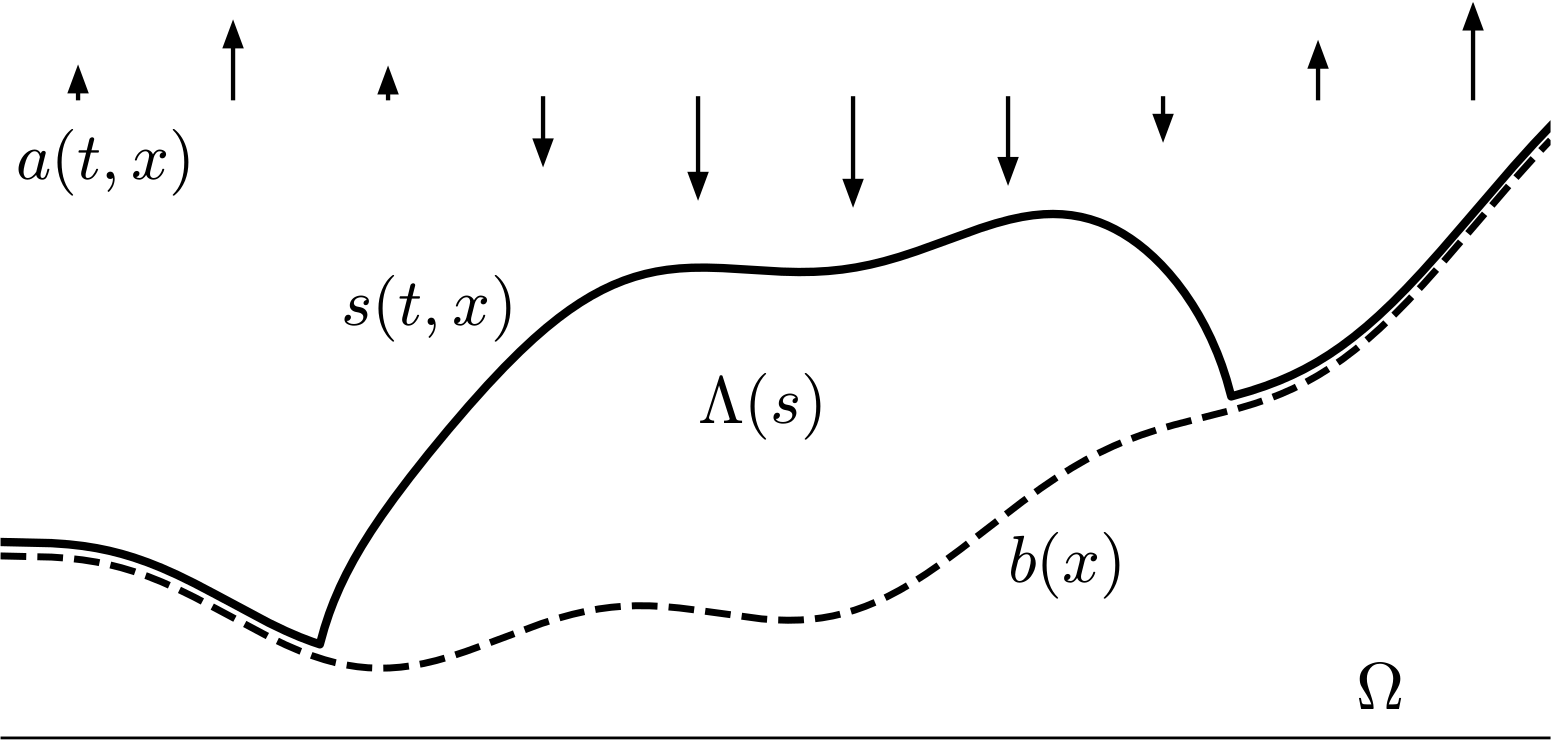
\includegraphics[width=0.6\textwidth]{genfigs/stokesdomain.pdf}
\caption{Glacier notation: $x\in\Omega\subset\RR^2$ and $\Lambda(t)\subset\RR^3$.}
\label{fig:stokesdomain}
\end{figure}

Let $s(t,x)$ be the (solution) ice surface elevation.  This is defined for all $x\in\Omega$, but subject to the constraint that the surface $z=s$ must be at or above the bedrock ($s \ge b$), and thus in regions with no ice $s=b$ holds.  The solution ice velocity $\bu(t,x,z)$ and pressure $p(t,x,z)$ are then defined only on the open 3D domain
\begin{equation}
\Lambda(t) = \left\{(x,z)\,:\,b(x) < z < s(t,x)\right\} \subset \Omega \times \RR. \label{eq:icydomain}
\end{equation}
This aspect of glacier modeling deserves emphasis:  The time-dependent 3D domain $\Lambda(t)$, on which the velocity and pressure are meaningful, is determined by the evolving surface elevation $s$, which is itself part of the coupled model solution.

The surface trace of the ice velocity will be of importance, and a precise Sobolev space for the velocity is given in Section \ref{sec:stokes}.  We extend it by zero so that it is defined for all $t,x \in [0,T]\times\Omega$; compare flux extension by zero in \cite{SchoofHewitt2013}:
\begin{equation}
\bu|_s(t,x) = \begin{cases} \bu(t,x,s(t,x)), & s(t,x)>b(t,x) \\
                            \bzero, & \text{otherwise} .\end{cases} \label{eq:defineus}
\end{equation}
Also let $\bn_s = \left<-\partial s/\partial x_1,-\partial s/\partial x_2,1\right>$ denote an upward surface normal vector, assumed well-defined for this Introduction.

The glacier geometry evolution model says that an infinite-dimensional nonlinear complementarity problem (NCP) \cite{FacchineiPang2003}, an obstacle problem, applies in $[0,T]\times \Omega$:
\begin{subequations}
\label{eq:ncp}
\begin{align}
s - b &\ge 0 \label{eq:ncp:constraint} \\
\frac{\partial s}{\partial t} - \bu|_s \cdot \bn_s - a &\ge 0 \label{eq:ncp:residualpos} \\
(s - b) \left(\frac{\partial s}{\partial t} - \bu|_s \cdot \bn_s - a\right) &= 0
\end{align}
\end{subequations}
While condition \eqref{eq:ncp:constraint} is sometimes stated in glacier literature \cite{Durandetal2009,Halfar1981,JouvetBueler2012,PiersantiTemam2023,WirbelJarosch2020}, the complementary fact \eqref{eq:ncp:residualpos}, that the residual is everywhere nonnegative, though observed in \cite{Calvoetal2003}, is rarely written \cite{SchoofHewitt2013}.

System \eqref{eq:ncp} implies that either a location is ice free ($s=b$), where the climate is locally ablating ($a\le 0$), or that the surface kinematical equation (SKE) holds:
\begin{equation}
\frac{\partial s}{\partial t} - \bu|_s \cdot \bn_s - a = 0.  \label{eq:ske}
\end{equation}
Equation \eqref{eq:ske} says that the (non-material) ice surface moves vertically according to the sum of an ice velocity component at the surface and the SMB.  This statement of mass conservation \cite{Aschwandenetal2012} is called the free-surface equation \cite{LofgrenAhlkronaHelanow2022} or kinematic boundary condition\footnote{Equation \eqref{eq:ske} is \emph{not}, however, a boundary condition for any identified PDE problem.} \cite{GreveBlatter2009}.  In numerical ice sheet models equation \eqref{eq:ske} is a standard way for surface geometry to evolve \cite{GreveBlatter2009,SchoofHewitt2013}, and glaciologists would agree with the conditions of NCP \eqref{eq:ncp}, but it is not common to state it completely in this way.  In any case, ice-free conditions are understood to exist only where (continuous) SMB is non-positive.

Because a simulated glacier needs to be able to advance into unglaciated locations, we assume that the SMB is defined everywhere in $\Omega$, regardless of whether a glacier is present or not.  In ice-free areas this input should have the value which a glacier surface would experience at that time and location.  It can be computed from precipitation and an energy balance model \cite{GreveBlatter2009}, for example by hypothesizing an ice surface and computing the balance of snow accumulation minus ablation which would follow from using the available energy for melt.

Additional to the kinematical considerations above, we must address the standard non-shallow ice dynamics model used in this paper.  It is the non-sliding (e.g.~frozen base), isothermal, non-Newtonian, and incompressible Stokes system \cite{GreveBlatter2009,JouvetRappaz2011,SchoofHewitt2013}, applied over the domain $\Lambda(t)$ defined in \eqref{eq:icydomain}.  Let $\Gamma_s(t)$, $\Gamma_b(t)$ denote the upper and lower surfaces $z=s$, $z=b$, respectively.  (The possibility of cliffs at the ice margin will be neglected, so $\partial \Lambda(t) = \overline{\Gamma_s(t)} \cup \overline{\Gamma_b(t)}$.)  To state the shear-thinning constitutive relationship in the model, Glen's flow law \cite{GreveBlatter2009}, let $D\bu=(\grad \bu + \grad \bu^{\top})/2$ denote the strain rate tensor, with Frobenius norm $|D\bu| = \left((D\bu)_{ij} (D\bu)_{ij}\right)^{1/2}$.  The effective dynamic viscosity \cite{GreveBlatter2009} of the ice is then given by a regularized formula
\begin{equation}
\nu(D\bu) = \nu_\pp \left(|D\bu|^2 + \mu_0\right)^{(\pp-2)/2} \label{eq:glen}
\end{equation}
for some $\mu_0>0$.  The exponent $1 < \pp \le 2$, written $\pp=(1/\nn)+1$ in terms of Glen's exponent $\nn\ge 1$, is commonly taken to be $\pp=4/3$ \cite{GreveBlatter2009}.  The coefficient $\nu_\pp>0$ has $\pp$-dependent units, while the result $\nu(D\bu)$ has SI units $\text{kg}\,\text{m}^{-1}\,\text{s}^{-1}$.  The values of $\nn$ and $\nu_\pp$ are constrained by laboratory experiments on ice \cite{GoldsbyKohlstedt2001,GreveBlatter2009}, and by temperature, but they are assumed to be constant here.  While $\pp=2$ for a Newtonian fluid with constant viscosity, if $\pp < 2$ then the regularization implies that $\nu(D\bu)$ is bounded.

At each time $t$ the velocity and pressure solve the following 3D fluid equations:%
\begin{subequations}
\label{eq:stokes}
\begin{align}
- \nabla \cdot \left(2 \nu(D\bu)\, D\bu\right) + \nabla p &= \rhoi \bg && \text{within $\Lambda(t)$} \\
\nabla \cdot \bu &= 0 && \qquad \text{''} \label{eq:stokes:incomp} \\
\left(2 \nu(D\bu) D\bu - pI\right) \bn_s &= \bzero && \text{on $\Gamma_s(t)$}\label{eq:stokes:stressfreesurface} \\
\bu  &= \bzero && \text{on $\Gamma_b(t)$} \label{eq:stokes:noslide}
\end{align}
\end{subequations}
The density of ice $\rhoi$ and the acceleration of gravity $\bg$ are assumed constant.  Boundary condition \eqref{eq:stokes:stressfreesurface} says that the sub-aerial upper surface is stress free.  Though both apply on $\Gamma_s(t)$,  \eqref{eq:stokes:stressfreesurface} must not be confused with equation \eqref{eq:ske}.

The Stokes sub-problem \eqref{eq:glen}, \eqref{eq:stokes} is commonly discretized using a finite element (FE) approximation  \cite{IsaacStadlerGhattas2015,Jouvetetal2008,Pattynetal2008}.  We will assume so in this paper.

In summary, at this point, we consider an evolving free-surface flow for a glacier, subject to a signed climate which can add or remove ice, simultaneously with a non-Newtonian Stokes problem which must be solved within the evolving 3D domain of ice.  This coupled initial-boundary value problem, in strong form as \eqref{eq:icydomain}--\eqref{eq:stokes}, requires data $b(x)$ and $a(t,x)$, plus an initial surface elevation $s(0,x)$.  The solution variables are $s(t,x)$, $\bu(t,x,z)$, and $p(t,x,z)$, with $s$ defined everywhere over $[0,T]\times \Omega$, subject to $s \ge b$, but with $\bu,p$ defined only on $\Lambda(t)$ given by \eqref{eq:icydomain}.

Observe that NCP \eqref{eq:ncp} is the only part of the model where a time derivative appears.  That is, because the flow is very viscous \cite{Acheson1990}, the Stokes sub-model acts as an instantaneous ``algebraic'' constraint on the evolution.  Therefore this coupled and infinite-dimensional problem is simultaneously a differential algebraic equation (DAE) system \cite{AscherPetzold1998,LofgrenAhlkronaHelanow2022} and a free-boundary, obstacle-type NCP.  While the coupled system is a standard physical model for a non-shallow evolving glacier, as a mathematical model it is poorly understood.  No well-posedness theory is known to this author, and in fact the current paper seems to be the first time that the model is stated with (proposed) function spaces for all variables, specifically including the surface elevation.

A formulation using ice thickness to parameterize glacier geometry would have a different character from the one using surface elevation here.  The surface elevation $s$ is subject to a flow-caused smoothing effect, illustrated for a real ice sheet in Figure \ref{fig:giscross}.  For land-based glaciers $s(t,x)$ is therefore generally smoother in $x$ than the thickness $H(t,x) = s(t,x)-b(x)$.  The thickness ``inherits'' the lower regularity of the often steep and eroded bedrock topography.

\begin{figure}
\begin{minipage}[t]{0.8\textwidth}
\vspace{0pt}
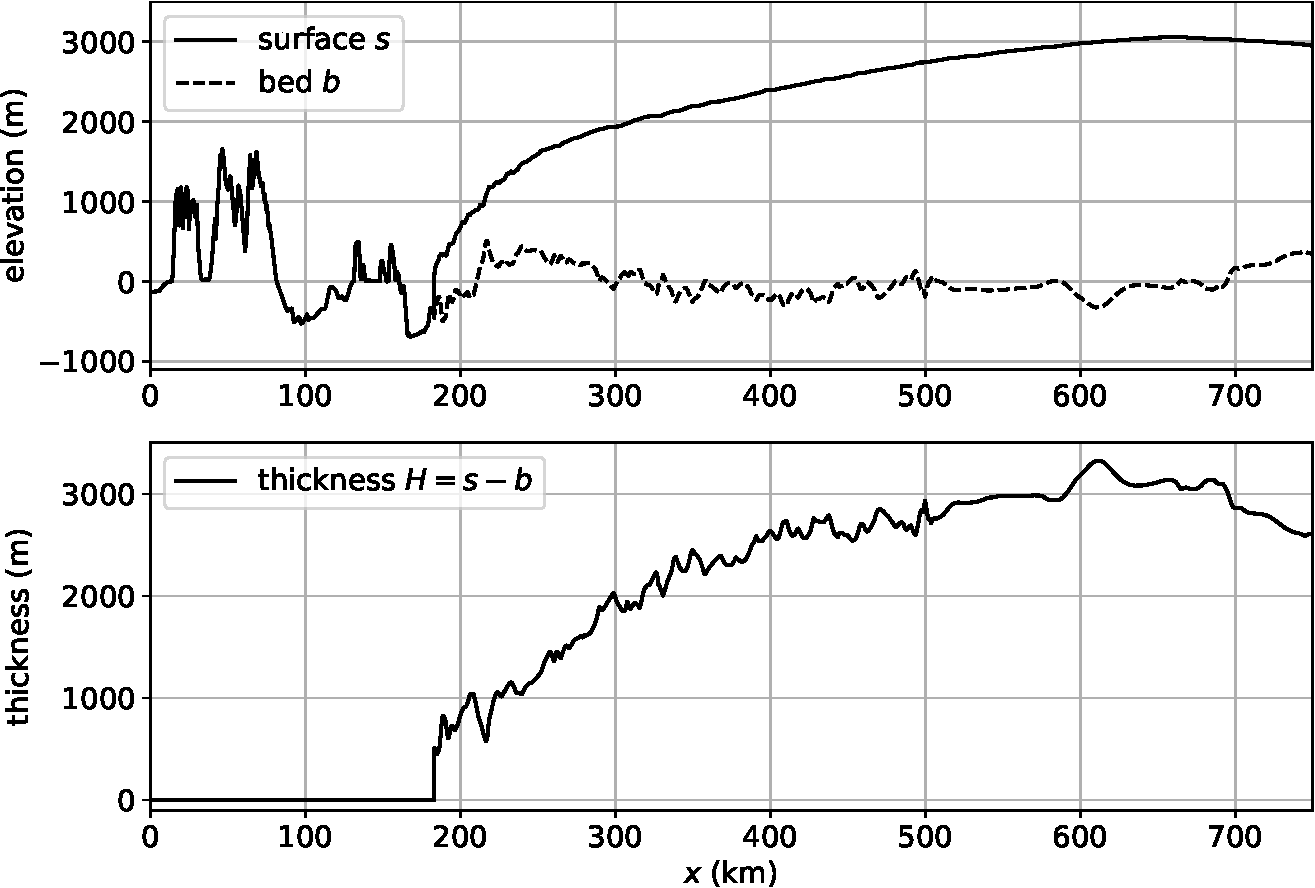
\includegraphics[width=\textwidth]{genfigs/giscross.pdf}
\end{minipage}
\,
\begin{minipage}[t]{0.15\textwidth}
\vspace{10pt}
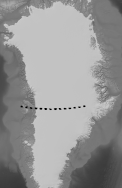
\includegraphics[width=\textwidth]{genfigs/gis/gris-profile-gray.png}
\end{minipage}
\caption{A cross-section of the Greenland ice sheet at $70^\circ$N latitude \cite{Morlighemetal2017}; see inset.  Top: While the ice surface $s$ is smoothed because of ice flow, the bedrock elevation $b$ is much rougher.  Bottom: The corresponding ice thickness $H = s-b$ inherits the low regularity of $b$.}
\label{fig:giscross}
\end{figure}

In this work we consider fully-implicit time stepping for NCP \eqref{eq:ncp}, as follows.  For a time step $\Delta t > 0$, and times $\{t_n\}$ with $t_n-t_{n-1}=\Delta t$, we apply a backward Euler semi-discretization scheme to \eqref{eq:ncp}, giving a new NCP for the updated surface elevation $s^n \approx s(t_n,x)$:
\begin{subequations}
\label{eq:be:ncp}
\begin{align}
s^n - b &\ge 0 \label{eq:be:ncp:constraint} \\
s^n - \Delta t\,\bu|_{s^n} \cdot \bn_{s^n} - \ell^n &\ge 0 \label{eq:be:ncp:residualpos} \\
(s^n - b) \left(s - \Delta t\,\bu|_{s^n} \cdot \bn_{s^n} - \ell^n\right) &= 0 \label{eq:be:ncp:complementarity}
\end{align}
\end{subequations}
For clarity we have collected a source term $\ell^n(x) = s^{n-1}(x) + \int_{t_{n-1}}^{t_n} a(t,x)\,dt$, with time-integrated climatic inputs.  In Section \ref{sec:model} we will re-write \eqref{eq:glen}--\eqref{eq:be:ncp} as a weak-form variational inequality (VI) for $s$ in an admissible subset of a Banach space.  Based on conjectured well-posedness for this problem (Section \ref{sec:conjectural}), our main results are new estimates on the numerical error in an FE approximation of the VI (Sections \ref{sec:abstractestimate}, \ref{sec:application}).

To the author's knowledge all existing evolution models using Stokes dynamics, or in any case with resolution of membrane stresses \cite{Bueler2023}, use an explicit or semi-implicit time-stepping scheme for the geometry \cite[for examples]{Brinkerhoff2023,Durandetal2009,Jouvetetal2008,LofgrenAhlkronaHelanow2022,WirbelJarosch2020}, or are fully-implicit only for a fixed map-plane region.\footnote{J.~Ahlkrona, personal communication.  Draft of: J.~Ahlkrona, A.~Löfgren, and C.~Henry (2025). \emph{A stable, fully implicit, second order method for viscous free surface Stokes flow}.}  That is, when partial implicitness is attempted, the part of $\RR^2$ covered by (solution) ice is not general.  Most schemes limit margin advance or retreat to one cell from the previous time step.  The current paper considers the full solution of a single time step of glacier evolution, computing the ice-covered area, and the surface elevation function, predicted from the data.

For finite-dimensional DAE systems, implicit schemes are the standard choice, that is, to handle stiffness \cite{AscherPetzold1998}.  In the infinite-dimensional case here, where NCP \eqref{eq:ncp} is constrained by the ``algebraic'' Stokes problem \eqref{eq:glen}--\eqref{eq:stokes}, implicit schemes are thus also the natural choice.  The backward Euler scheme \eqref{eq:be:ncp} is the simplest A-stable scheme \cite{AscherPetzold1998} which can be applied.  Extension to higher-order A-stable and stiff decay schemes \cite{AscherPetzold1998} is natural.  However, \eqref{eq:glen}--\eqref{eq:be:ncp} already contains all important features.

A (fully) explicit version of \eqref{eq:be:ncp} would replace $s^n$ in the surface motion term by the previous surface elevation: $\bu|_{s^n} \cdot \bn_{s^n} \to \bu|_{s^{n-1}} \cdot \bn_{s^{n-1}}$ \cite{Lengetal2012}.  One semi-implicit scheme uses the surface velocity from the old time, but with the updated value for the surface slope part: $\bu|_{s^n} \cdot \bn_{s^n} \to \bu|_{s^{n-1}} \cdot \bn_{s^n}$ \cite{Durandetal2009}.  A different form of semi-implicitness comes from modifying the body force in the Stokes problem using an explicit surface estimate \cite{LofgrenAhlkronaHelanow2022}.  These schemes are not the same as implicit scheme \eqref{eq:be:ncp}.

One may make a case for implicit time-stepping based on simulation performance, that is, by applying computational complexity scaling arguments which compare to various conditionally-stable explicit alternatives \cite{Bueler2023}.  However, actual performance advantages will depend on positive answers to the key questions:  Is the implicit-step VI problem well-posed?  Can it be solved accurately and efficiently?  Does the (coupled) implicit scheme have unconditional stability?  In the current paper we address well-posedness and FE accuracy.  Solver efficiency and time-stepping stability are topics for further research.

This paper is organized as follows.  Section \ref{sec:stokes} recalls the theory of the Glen-law Stokes problem on a fixed 3D domain.  For this sub-model we give a new bound on the surface trace of the velocity solution (Corollary \ref{cor:surfacetracebound}).  In Section \ref{sec:model} we re-formulate the coupled, implicit-step NCP problem \eqref{eq:glen}--\eqref{eq:be:ncp} as a VI weak form.  The key coupling is the implicit surface motion term $\bu|_{s^n}\cdot \bn_{s^n}$.  For this term we provide a quantitative bound over a Sobolev space of surface elevation functions (Lemma \ref{lem:philipschitz}), subject to Conjectures \ref{conj:a} and \ref{conj:b}.  Well-posedness for each implicit step VI problem, and the operator coercivity needed to apply the later \emph{a priori} bound on the FE solution, is then considered in Section \ref{sec:conjectural}.  Certain physical and modeling ideas are the context needed to understand Conjecture \ref{conj:c}, which hypotheses the coercivity of a regularization of this surface motion term.  Numerical results support this major Conjecture.  While well-posedness is conjectural, no prior attempt to formulate a mathematical coupled, non-shallow, free-boundary glacier model is known to the author, and thus such a continuum model is here stated precisely for the first time.

With this temporally semi-discretized model in hand, we then turn to results on numerical approximations in space.  In Section \ref{sec:abstractestimate} we prove an abstract FE error estimate, Theorem \ref{thm:abstractestimate} and its Corollaries, which are apparently new at this level of generality, namely for VI problems involving nonlinear operators on Banach spaces.  This estimate, which makes coercivity and Lipshitz assumptions on the operator, extends a classical bilinear argument by Falk \cite{Falk1974}.  In Section \ref{sec:application} we apply the abstract estimate to the glacier problem, yielding our main result which is Theorem \ref{thm:glacierapp}.  The physical significance of each term in this error estimate, and how associated FE method and glacier modeling choices can be made, is addressed at the end.

We will use only the following few abbreviations which are standard in their respective fields: DAE (differential-algebraic equations), FE (finite element), NCP (nonlinear complementarity problem), PDE (partial differential equation), SKE (surface kinematical equation), SMB (surface mass balance), and VI (variational inequality).


\section{Surface velocity from the Stokes sub-model} \label{sec:stokes}

In this Section we address only the Stokes sub-model \eqref{eq:glen}--\eqref{eq:stokes}, applied at some time $t$, that is, on a (for now) fixed 3D domain $\Lambda = \Lambda(t)$ defined by \eqref{eq:icydomain}.  The ice base $\Gamma_b\subset\partial \Lambda$, on which the non-sliding Dirichlet condition \eqref{eq:stokes:noslide} holds, is assumed to have positive measure.  The remaining Neumann boundary $\Gamma_s = \partial \Lambda \setminus \overline{\Gamma_b}$ is subject to a zero normal stress condition \eqref{eq:stokes:stressfreesurface}.  This submodel will compute the surface velocity $\bu|_s$ which appears in NCPs \eqref{eq:ncp} and \eqref{eq:be:ncp}, but we defer this coupling to later sections.

Suitable function spaces for well-posedness of this sub-model are known.  Let $1 < \pp \le 2$.  Denote the Sobolev space \cite{Evans2010} of real-valued functions on $\Lambda \subset \RR^3$ with $\pp$th-power integrable first derivatives by $W^{1,\pp}(\Lambda)$, and let $\cV = W_0^{1,\pp}(\Lambda; \RR^3)$ be the corresponding space of vector-valued functions with trace zero along $\Gamma_b$.  Let $[H]\ge 1\,\text{meter}$ be a representative \emph{vertical} glacier scale.  We define the norm on $\cV$ by
\begin{equation}
\|\bv\|_{\cV} = \left(\int_\Lambda |\bv|^\pp\,dx\,dz + [H]^\pp \int_\Lambda |\grad\bv|^\pp\,dx\,dz\right)^{1/\pp}. \label{eq:vnorm}
\end{equation}
(The 3D volume element $dx\,dz = dx_1\,dx_2\,dz$ will be suppressed from now on.)  Here $|\bv|$ denotes the Euclidean norm, $|\grad\bv|=\left((\grad\bv)_{ij} (\grad\bv)_{ij}\right)^{1/2}$ is the Frobenius norm on $\RR^{3\times 3}$, and the scale $[H]$ gives $\|\bv\|_{\cV}$ consistent units; compare \cite[Remark 1.2.1]{BoffiBrezziFortin2013}.  Let $\cQ=L^{\pp'}(\Lambda)$ where $\pp'=\pp/(\pp-1)$ is the conjugate exponent.  Define $\mathcal{M} = \cV \times \cQ$ as the space of admissible velocity and pressure pairs.  For $(\bu,p), (\bv,q) \in \mathcal{M}$ define
\begin{equation}
F_\Lambda(\bu,p)[\bv,q] = \int_\Lambda 2 \nu(D\bu) D\bu : D\bv - p \Div\bv - (\Div\bu) q - \rhoi \bg \cdot \bv, \label{eq:glenstokes:fcnl}
\end{equation}
where $A:B=a_{ij}b_{ij}$.  The (mixed) weak form of the Stokes sub-model \eqref{eq:glen}--\eqref{eq:stokes} seeks the solution $(\bu,p) \in \mathcal{M}$ satisfying
\begin{equation}
F_\Lambda(\bu,p)[\bv,q] = 0 \qquad \text{for all } (\bv,q) \in \mathcal{M}. \label{eq:glenstokes:weak}
\end{equation}

Jouvet and Rappaz \cite{JouvetRappaz2011} have proven that problem \eqref{eq:glenstokes:weak} is well-posed if the Neumann portion of $\partial\Lambda$ is piecewise $C^1$.  Their proof of the following theorem uses the equivalence of \eqref{eq:glenstokes:weak} and a minimization problem over the divergence-free subspace $\cV_0 = \{\bv\in\cV\,:\,\Div\bv=0\}$.  Our regularization in Glen law \eqref{eq:glen} differs from theirs, but the necessary modifications are addressed in \cite{Belenkietal2012,IsaacStadlerGhattas2015}.  Note that if the weak solution is sufficiently regular then the strong form \eqref{eq:stokes} is also satisfied.

\begin{theorem}[Theorem 3.10 in \cite{JouvetRappaz2011}] \label{thm:stokeswellposed}  Suppose $\Lambda$ is bounded, $\partial\Lambda$ is Lipschitz, $\Gamma_s$ is piecewise $C^1$, and $\Gamma_b$ has positive measure.  Let $1<\pp\le 2$ and $\mu_0>0$ in \eqref{eq:glen}.  Then there exists a unique pair $(\bu,p) \in \mathcal{M}$ solving \eqref{eq:glenstokes:weak}, and $\bu\in \cV_0$.
\end{theorem}

Our primary purpose is to study NCP \eqref{eq:be:ncp} for glacier geometry, and its weak form, but for that we need control on the surface trace $\bu|_s$.  The following \emph{a priori} bound is proven for completeness in Appendix \ref{app:provestokesapriori}.

\begin{lemma} \label{lem:stokesapriori}
There is $C>0$ depending continuously on $\pp$, $\rhoi |\bg|$, $\nu_\pp$, $\mu_0$, $[H]$, and $\Lambda$ so that if $\bu\in\cV_0$ is the solution from Theorem \ref{thm:stokeswellposed} then
\begin{equation}
\|\bu\|_{\cV} \le C. \label{eq:stokesapriori}
\end{equation}
\end{lemma}

\begin{lemma}[Trace inequality] \label{lem:trace}
Under the assumptions of Theorem \ref{thm:stokeswellposed}, there exists a constant $C$, dependent only on $\pp$, $[H]$, and $\Lambda$, so that for all $\bv \in \cV$,
\begin{equation}
\int_{\Gamma_s} \big|\bv|_s\big|^\pp \,dS \le C \|\bv\|_{\cV}^\pp. \label{eq:trace}
\end{equation}
On the left of \eqref{eq:trace}, $\bv|_s$ denotes the trace on $\Gamma_s$ and $dS$ is the area element over $\partial\Lambda$.
\end{lemma}

\begin{proof}
Theorem 5.5.1 in \cite{Evans2010} defines the trace operator $T:\cV\to L^\pp(\partial\Lambda)$, for which there exists a constant $c>0$ so that
\begin{equation}
\int_{\partial\Lambda} |T\bv|^p\,dS \le c \int_{\Lambda} |\bv|^\pp + |\grad\bv|^\pp \le c \int_{\Lambda} |\bv|^\pp + [H]^\pp |\grad\bv|^\pp \label{eq:tracework}
\end{equation}
for $\bv\in\cV$.  However, because $\bv=\bzero$ along $\Gamma_b$, the result follows.
\end{proof}

Combining Lemmas \ref{lem:stokesapriori} and \ref{lem:trace} yields the following bound on the surface trace of the velocity.  When applying this result, recall that $\Lambda=\Lambda(t)$ and $\Gamma_s=\Gamma_s(t)$ are defined via \eqref{eq:icydomain}, in terms of $s(t,x)$ and $b(x)$.

\begin{corollary}[\emph{A priori} surface velocity bound] \label{cor:surfacetracebound}
Under the assumptions of Theorem \ref{thm:stokeswellposed}, there is a constant $C>0$, computable from physical constants and the geometry of $\Lambda$, so that if $\bu\in\cV_0$ is the Stokes velocity solution then
\begin{equation}
\int_{\Gamma_s} \big|\bu|_s\big|^\pp \,dS \le C. \label{eq:surfacetracebound}
\end{equation}
\end{corollary}


\section{The weak form of an implicit time step} \label{sec:model}

Now we return to implicit time steps for glacier geometry evolution.  Let $t_n$ denote increasing times in $[0,T]$, with $t_0=0$ and $\Delta t = t_n-t_{n-1}$ denoting a generic step duration.  Let $a^n(x)$ be the average of the data $a(t,x)$ over $[t_{n-1},t_n]$.  Suppose that $s^n(x)\approx s(t_n,x)$ approximates the surface elevation at time $t_n$.  The backward Euler scheme \cite{AscherPetzold1998} for SKE \eqref{eq:ske} is
\begin{equation}
\frac{s^n - s^{n-1}}{\Delta t} - \bu|_{s^n} \cdot \bn_{s^n} - a^n = 0. \label{eq:be:ske}
\end{equation}
This scheme is fully-implicit because the unknown $s^n$ appears both in the surface velocity $\bu|_{s^n}$ and in the slope $\bn_{s^n}$.

For cleaner appearance we will write $s=s^n$ for the unknown surface elevation, and we collect a source term, defined over all of $\Omega$:
\begin{equation}
\boxed{\ell^n(x) = s^{n-1}(x)+\Delta t\,a^n(x) = s^{n-1}(x) + \int_{t_{n-1}}^{t_n} a(t,x)\,dt.} \label{eq:be:source}
\end{equation}

As noted in the Introduction, $s$ solves a problem of free-boundary type at time $t_n$, namely NCP \eqref{eq:be:ncp}, which says that either there is bare ground ($s=b$) or equation \eqref{eq:be:ske} holds.  A weak-form variational inequality (VI; \cite{Evans2010,KinderlehrerStampacchia1980}) version of this problem is better-suited in theory and for finite element (FE) analysis.  Leaving the precise Banach space $\cX$ undecided, pending discussion below, admissible surface elevations for the weak formulation come from a convex and closed subset, a cone:
\begin{equation}
\boxed{\cK = \left\{\sigma \in\cX\,:\,\sigma|_{\partial\Omega}=b|_{\partial\Omega} \text{ and } \sigma \ge b\right\}.}  \label{eq:be:admissible}
\end{equation}
Note that a Dirichlet boundary condition is included in the definition of $\cK$.  We assume throughout that $b\in C^1(\bar\Omega)$ is smooth, with bounded gradient.  Now the VI form is derived by assuming that $s \in \cK$ is a sufficiently-regular solution of \eqref{eq:be:ncp}.  Let $\Omega_I = \{x\in\Omega\,:\,s(x)>b(x)\}$ be the (measurable) subset on which the constraint \eqref{eq:be:ncp:constraint} is inactive, i.e.~where glacier ice is present.  By \eqref{eq:be:ncp:constraint}, integration over $\Omega_I$ gives%
\begin{equation}
\int_{\Omega_I} \left(s - \Delta t\,\bu|_s \cdot \bn_s - \ell^n\right)\,(\sigma-s) = 0  \label{eq:inactivetruth}
\end{equation}
for any $\sigma\in\cK$.  On the other hand, let $\Omega_A = \Omega \setminus \Omega_I$ be the active (ice-free) region.  Using extension by zero \eqref{eq:defineus}, inequality \eqref{eq:be:ncp:residualpos} over $\Omega_A$ implies $b-\ell^n = s - \Delta t\,\bu|_s \cdot \bn_s - \ell^n \ge 0$.  Since also $\sigma-s=\sigma-b\ge 0$ on $\Omega_A$, integration yields an inequality:
\begin{equation}
\int_{\Omega_A} \left(s - \Delta t\,\bu|_s \cdot \bn_s - \ell^n\right)\,(\sigma-s) = \int_{\Omega_A} \left(b - \ell^n\right)\,(\sigma-b) \ge 0.  \label{eq:activetruth}
\end{equation}
Adding \eqref{eq:inactivetruth} and \eqref{eq:activetruth} gives
\begin{equation}
\int_\Omega \left(s - \Delta t\,\bu|_s \cdot \bn_s - \ell^n\right)\,(\sigma-s) \ge 0 \quad \text{for all } \sigma \in \cK. \label{eq:be:viearly}
\end{equation}
This VI is true for $s\in\cK$, in advance of knowing which part of $\Omega$ is ice-covered.

It remains to identify a Sobolev space $\cX$ suitable for admissible surface elevations.  Within a Stokes-based theory, the shape that should be predicted for a glacier's grounded margin is not clear (Figure \ref{fig:margins}).  ``Wedge'' shapes with bounded gradients have been hypothesized from observations \cite{EchelmeyerKamb1986}, while shallow-ice theory suggests root-type (fractional-power) shapes, with different powers for advance and retreat \cite{Bueleretal2005,JouvetBueler2012}.  However, in real glacier margins the ice can overhang, especially on steep bedrock features, violating our assumption of a single-valued surface elevation.  The bedrock itself can overhang, and fractures, crevasses, and cliffs are common.

\begin{figure}[ht]
\begin{center}
\begin{tikzpicture}[scale=1.0]
  \node (wedge) {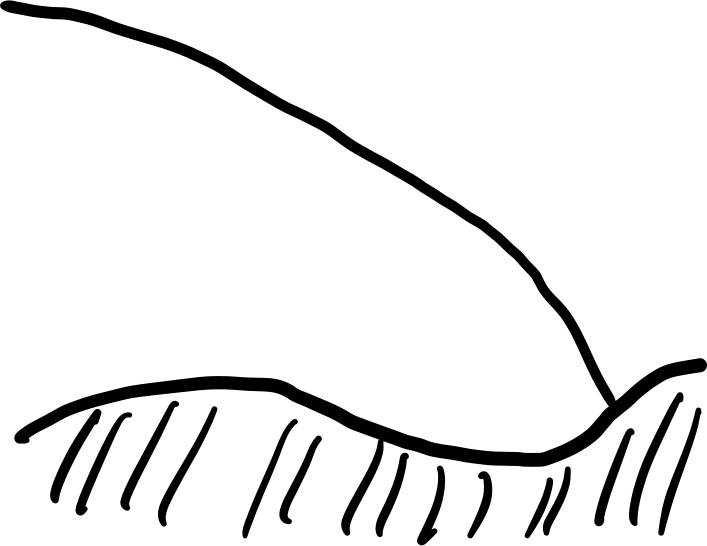
\includegraphics[width=30mm]{figs/wedge.png}} node[xshift=-4mm, yshift=1mm] at (wedge.center) {{\small \emph{ice}}};
  \node[right=of wedge] (unbounded) {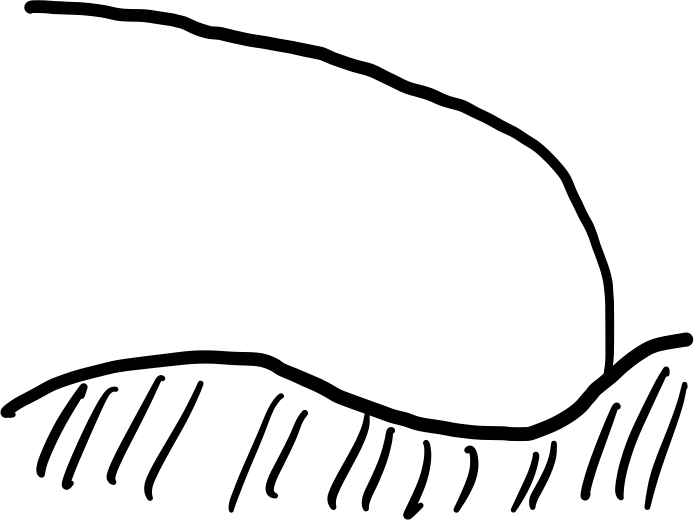
\includegraphics[width=30mm]{figs/unbounded.png}} node[xshift=-2mm, yshift=1mm] at (unbounded.center) {{\small \emph{ice}}};
  \node[right=of unbounded] (realistic) {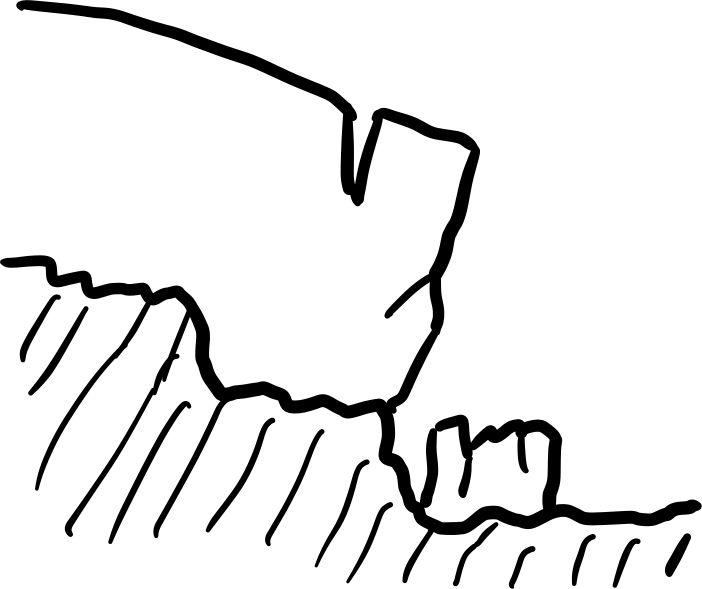
\includegraphics[width=30mm]{figs/realistic.png}} node[xshift=-6mm, yshift=4mm] at (realistic.center) {{\small \emph{ice}}};
\end{tikzpicture}
\end{center}

\vspace{-2mm}

\caption{Glacier margins with finite-slope ``wedge'' shapes (left) are possible, while shallow theory has fractional powers (center).  Actual glacier margins have overhangs and fractures (right).}
\label{fig:margins}
\end{figure}

Major numerical models all ignore overhangs \cite{IsaacStadlerGhattas2015,Jouvetetal2008,LofgrenAhlkronaHelanow2022,WirbelJarosch2020},
and fractures cannot occur within the viscous-fluid paradigm in such models.  We will follow these conventions.  Though clearly beyond our scope, future models might allow fractures, supplementing momentum conservation with an advected damage variable and a stress-failure criterion \cite{PralongFunk2005}.  Averaged over hundred-meter scale, the resulting emergent margin shapes might suggest a regularity assumption within the viscous theory, and thus a Sobolev space for surface elevations.

For now we attempt to choose $\cX$ based on mathematical considerations within the viscous theory.  Our main idea is that well-posedness of the weak-form Stokes problem \eqref{eq:glenstokes:weak}, plus the surface trace bound in Corollary \ref{cor:surfacetracebound}, allows us to create a well-defined map from an admissible surface elevation $s\in \cK$ to the surface motion term $\bu|_s\cdot \bn_s$ in \eqref{eq:be:viearly}.  However, to properly understand this map we change 3D domain notation.  The ice domain depends only on the surface elevation, so we write
\begin{equation}
\boxed{\Lambda(s) = \left\{(x,z)\,:\,b(x) < z < s(x)\right\} \subset \Omega \times \RR,} \label{eq:domainfroms}
\end{equation}
within the implicit time step problem, replacing the time-dependent case \eqref{eq:icydomain}.  Now, for a given input $s\in\cK$, the map solves the Stokes model \eqref{eq:glenstokes:weak} over $\Lambda(s)$, then evaluates the trace of $\bu$ along $\Gamma_s$ (Corollary \ref{cor:surfacetracebound}), then extends by zero, namely definition \eqref{eq:defineus}, and finally multiplies by $\bn_s$.

For this map to be defined, $s$ must be sufficiently-regular so that the Stokes problem has a solution $\bu$ with a surface trace, and this constrains the choice of $\cX$.  In fact, the term $\bu|_s\cdot \bn_s$ in \eqref{eq:be:viearly} is in the dual space $(W^{1,\rr}(\Omega))'$ if $s\in W^{1,\rr}(\Omega)$.  Let $[L]>0$ be a representative \emph{horizontal} scale for $\Omega\subset\RR^2$.  For $\omega\in W^{1,\rr}(\Omega)$ define
\begin{equation}
\|\omega\|_{W^{1,\rr}} = \left(\int_\Omega |\omega|^\rr\,dx + [L]^\rr \int_\Omega |\grad \omega|^\rr\,dx\right)^{1/\rr}; \label{eq:norm:Omega}
\end{equation}
compare \eqref{eq:vnorm}.  The following preliminary bound assumes that $s \in W^{1,\rr}(\Omega)$ is nice enough for Theorem \ref{thm:stokeswellposed} to apply.  The conclusion is that the measurable function $\bu|_s\cdot \bn_s$ is controlled, as it is an element of a dual space.

\begin{lemma}[Preliminary bound on surface motion] \label{lem:phibound:early}  Suppose $2 \le \rr \le \infty$ and that $s\in W^{1,\rr}(\Omega)$ satisfies $s\ge b$ and $s=b$ on $\partial\Omega$.  If $\Lambda(s)$, defined by \eqref{eq:domainfroms}, satisfies the hypotheses of Theorem \ref{thm:stokeswellposed} then there is $C(s)>0$ so that for all  $\omega\in W^{1,\rr}(\Omega)$,
\begin{equation}
\left|\int_\Omega \bu|_s\cdot \bn_s \,\omega\,dx\right| \le C(s)\, \|\omega\|_{W^{1,\rr}}. \label{eq:phibound:early}
\end{equation}
\end{lemma}

\begin{proof}  Recall that $dS = |\bn_s|\,dx = \sqrt{1+|\grad s|^2}\,dx$ is the surface area element for $\Gamma_s \subset \partial \Lambda$.  Apply H\"older's inequalities:
\begin{align}
\Big|\int_\Omega \bu|_s\cdot \bn_s \, &\omega\,dx\Big| \le \int_\Omega \big|\bu|_s\big| |\bn_s|^{1/\pp} |\bn_s|^{1/\pp'} |\omega|\,dx \label{eq:phibound:zero} \\
    &\le \left(\int_\Omega \big|\bu|_s\big|^\pp |\bn_s|\,dx\right)^{1/\pp} \left(\int_\Omega |\bn_s| |\omega|^{\pp'} \,dx\right)^{1/\pp'} \notag \\
    &\le \left(\int_{\Gamma_s} |\bu|^\pp \,dS\right)^{1/\pp} \left(\int_\Omega |\bn_s|^\rr \,dx\right)^{1/(\pp'\rr)} \left(\int_\Omega |\omega|^{\pp'\rr'} \,dx\right)^{1/(\pp'\rr')}. \notag
\end{align}
From bound \eqref{eq:surfacetracebound} we may write
\begin{equation}
\left|\int_\Omega \bu|_s\cdot \bn_s \, \omega\,dx\right| \le C \left(\int_\Omega \left(1+|\grad s|^2\right)^{\rr/2}\,dx\right)^{1/(\pp'\rr)} \|\omega\|_{L^{\pp'\rr'}}.
\end{equation}
Note that if $\alpha\ge 0$ then $(1+\alpha)^{\rr/2} \le 2^{(\rr-2)/2} (1+\alpha^{\rr/2})$, so, using generic constants,
\begin{align}
\left|\int_\Omega \bu|_s\cdot \bn_s \, \omega\,dx\right| &\le C \left(2^{(\rr-2)/2} \int_\Omega 1 + |\grad s|^\rr\,dx\right)^{1/(\pp'\rr)} \|\omega\|_{L^{\pp'\rr'}} \label{eq:phibound:one} \\
  &\le C \left(|\Omega| + [L]^{-\rr}\|s\|_{W^{1,\rr}}^\rr\right)^{1/(\pp'\rr)} \|\omega\|_{L^{\pp'\rr'}}. \notag
\end{align}
Since $2 \le \pp' \le \pp'\rr' < \infty$, by Sobolev's inequality, e.g.~Theorem 8.8 from \cite{LiebLoss1997} using $n=2$, $k=m=1$, $p=\rr$, and $\omega=\pp'\rr'$, we have $\|\omega\|_{L^{\pp'\rr'}} \le C \|\omega\|_{W^{1,\rr}}$, thus \eqref{eq:phibound:early}.
\end{proof}

Because $\Omega\subset \RR^2$, if $\rr>2$ then $W^{1,\rr}(\Omega) \hookrightarrow C(\bar\Omega)$.  However, for $s\in W^{1,\rr}(\Omega)$, generally $\Gamma_s\subset \Lambda(s)$ is not piecewise $C^1$ as stated in the hypotheses of Theorem \ref{thm:stokeswellposed}.  We conjecture that nonetheless $\Lambda(s)$ is a domain on which the Stokes sub-model \eqref{eq:glenstokes:weak} is well-behaved enough for the construction of our map from $s$ to the surface motion term $\bu|_s\cdot \bn_s$.  Note that in Section \ref{sec:application} the FE approximation $s_h\approx s$ will be continuous and piecewise-linear---see Figure \ref{fig:fe:operatorvisualization}---so Theorem \ref{thm:stokeswellposed} will hold on the domain $\Lambda(s_h)$.

\begin{conjecture}[$W^{1,\rr}$ surface elevations allow Stokes solutions] \label{conj:a}
There exists $2 < \rr \le \infty$ so that if $s\in W^{1,\rr}(\Omega)$ is admissible then the conclusion of Theorem \ref{thm:stokeswellposed} applies on $\Lambda(s)$, providing a unique pair $(\bu,p) \in \mathcal{M}$ solving \eqref{eq:glenstokes:weak}, with $\bu\in \cV_0$.
\end{conjecture}

Suppose Conjecture \ref{conj:a} holds for some $\rr>2$.  Define
\begin{equation}
\boxed{\cX = W^{1,\rr}(\Omega),} \label{eq:defineX}
\end{equation}
with the admissible subset $\cK \subset \cX$ defined by \eqref{eq:be:admissible}.  By Corollary \ref{cor:surfacetracebound} the surface velocity $\bu|_s$ is well-defined as a measurable function, and its $L^\pp(\Gamma_s)$ norm is bounded.  By Lemma \ref{lem:phibound:early} the surface motion term $\bu|_s\cdot\bn_s$ is in $\cX'$.  However, to proceed with well-posedness we must further conjecture that a norm of $\bu|_s$, including extension-by-zero \eqref{eq:defineus}, is Lipschitz as a function of $s$.  Proving this might require more detailed knowledge about Stokes problem \eqref{eq:glenstokes:weak} than is currently available.

\begin{conjecture}[Surface velocity is Lipschitz in the surface elevation] \label{conj:b}
There exists $2 < \rr \le \infty$ so that if $R>0$ then there is $C(R)>0$ so that for $\sigma,s\in B_R \cap \cK = \{t\in \cK\,:\,\|t\|_{\cX} \le R\}$ we have
\begin{equation}
\big\|\bu|_\sigma - \bu|_s\big\|_{L^{\rr'}} \le C(R) \|\sigma-s\|_{\cX} \label{eq:ulipschitz}
\end{equation}
\end{conjecture}

From now on we will assume that Conjectures \ref{conj:a} and \ref{conj:b} hold for some $\rr>2$.

\begin{definition}  Define the nonlinear \emph{surface motion map} $\Phi:\cK \to \cX'$ by
\begin{equation}
\boxed{\Phi(s)[\omega] = -\int_\Omega \bu|_s\cdot\bn_s\,\omega\,dx,} \label{eq:definePhi}
\end{equation}
for $\omega\in \cX$.
\end{definition}

\begin{lemma} \label{lem:philipschitz}  The map $\Phi$ is Lipschitz on bounded subsets of $\cK$, that is, if $R>0$ then there is $\tilde C(R)>0$ so that for $\sigma,s\in B_R \cap \cK$ we have
\begin{equation}
\left\|\Phi(\sigma) - \Phi(s)\right\|_{\cX'} \le \tilde C(R)\, \|\sigma-s\|_{\cX}.  \label{eq:philipschitz}
\end{equation}
\end{lemma}

\begin{proof}  Let $R>0$ and assume without loss of generality that $R\ge \|b\|_\cX$, so $b\in B_R \cap \cK$.  Suppose $\sigma,s\in B_R \cap \cK$.  For any $\omega\in\cX$, in the following we add and subtract $\bu|_s \cdot \bn_\sigma$, and use the triangle inequality $|\bn_\sigma|=\left(1+|\grad \sigma|^2\right)^{1/2} \le 1 + |\grad \sigma|$:
\begin{align}
\Big|\Phi(\sigma)[\omega] - \Phi(s)[\omega]\Big| &\le \int_\Omega \Big|\bu|_\sigma - \bu|_s\Big| |\bn_\sigma| |\omega|\,dx + \int_\Omega \big|\bu|_s\big| |\bn_\sigma-\bn_s| |\omega|\,dx \\
    &\le \int_\Omega \Big|\bu|_\sigma - \bu|_s\Big| |\omega|\,dx + \int_\Omega \Big|\bu|_\sigma - \bu|_s\Big| |\grad \sigma| |\omega|\,dx \notag \\
    &\qquad\qquad + \int_\Omega \big|\bu|_s\big| |\grad \sigma-\grad s| |\omega|\,dx \notag
\end{align}
By applying H\"older's inequality to each of these integrals we have
\begin{align}
\int_\Omega \Big|\bu|_\sigma - \bu|_s\Big| |\omega|\,dx &\le \big\|\bu|_\sigma - \bu|_s\big\|_{L^{\rr'}} \|\omega\|_{L^{\rr}} \le \|\bu|_\sigma - \bu|_s\|_{L^{\rr'}} \|\omega\|_{\cX}, \label{eq:philipschitz:1} \\
\int_\Omega \Big|\bu|_\sigma - \bu|_s\Big| |\grad \sigma| |\omega|\,dx &\le \left(\int_\Omega \Big|\bu|_\sigma - \bu|_s\Big|^{\rr'} |\omega|^{\rr'}\, dx\right)^{1/\rr'} \|\grad \sigma\|_{L^\rr} \label{eq:philipschitz:2} \\
    &\le [L]^{-1} \big\|\bu|_\sigma - \bu|_s\big\|_{L^{\rr'}} \|\sigma\|_{\cX} \|\omega\|_{L^\infty}, \notag \\
\int_\Omega \big|\bu|_s\big| |\grad \sigma-\grad s| |\omega|\,dx &\le \left(\int_\Omega \big|\bu|_s\big|^{\rr'} |\omega|^{\rr'}\, dx\right)^{1/\rr'} \|\grad \sigma- \grad s\|_{L^\rr}  \label{eq:philipschitz:3} \\
    &\le [L]^{-1} \big\|\bu|_s - \bzero\big\|_{L^{\rr'}} \|\sigma-s\|_{\cX} \|\omega\|_{L^\infty}. \notag
\end{align}
Note that $\bu|_b=\bzero$; there is no flow when there is no glacier.  Because $\rr>2$, Sobolev's inequality gives $\|\omega\|_{L^\infty} \le c_\infty \|\omega\|_\cX$ for some $c_\infty>0$.  Now apply Conjecture \ref{conj:b} to each of \eqref{eq:philipschitz:1}--\eqref{eq:philipschitz:3}:
\begin{equation}
\big|\Phi(\sigma)[\omega] - \Phi(s)[\omega]\big| \le C(R) \left(1 + c_\infty [L]^{-1} \left(\|\sigma\|_{\cX} + \|s - b\|_{\cX}\right)\right) \|\sigma-s\|_{\cX} \|\omega\|_{\cX}.
\end{equation}
Recalling that $b\in B_R\cap \cK$, use the triangle inequality again to show that \eqref{eq:philipschitz} holds with $\tilde C(R) = C(R) \left(1 + 3 c_\infty [L]^{-1} R\right)$.
\end{proof}

At this point we have the tools needed to make the continuum model for a backward-Euler time-step \eqref{eq:be:ske} mathematically precise.

\begin{definition} For $\Delta t>0$, $s\in\cK$, and $\omega\in\cX$ define the nonlinear (Stokes) \emph{geometry update operator} $F_{\Delta t}:\cK\to\cX'$ as
\begin{equation}
\boxed{F_{\Delta t}(s)[\omega] = \Delta t\,\Phi(s)[\omega] + \int_\Omega s \omega.}  \label{eq:be:Fdefine}
\end{equation}
Assume that $\ell^n$, defined from data $s^{n-1}$ and $a$ by \eqref{eq:be:source}, is in $\cX'$.  We say that the surface elevation $s=s^n \in \cK$ solves the (weak-form) \emph{implicit time-step problem} if
\begin{equation}
\boxed{F_{\Delta t}(s)[\sigma-s] \ge \ell^n[\sigma-s] \quad \text{for all } \sigma \in \cK.} \label{eq:be:vi}
\end{equation}
\end{definition}

If Conjectures \ref{conj:a} and \ref{conj:b} hold then $F_{\Delta t}$ is well-defined and Lipschitz on bounded subsets (Lemma \ref{lem:philipschitz}).  The reader should confirm that VI \eqref{eq:be:vi} merely rewrites \eqref{eq:be:viearly}.  This weak form VI gives the precise meaning of strong-form NCP \eqref{eq:be:ncp}.

The seven boxed definitions and inequalities above, namely \eqref{eq:be:source}, \eqref{eq:be:admissible}, \eqref{eq:domainfroms}, \eqref{eq:defineX}, \eqref{eq:definePhi}, \eqref{eq:be:Fdefine}, and \eqref{eq:be:vi}, form a continuum model for a time step of glacier evolution based on Stokes dynamics.  Though conjectures are used in the construction of the operator $F_{\Delta t}$, this model is precise enough to be subject to mathematical analysis, including a future existence and uniqueness result.  However, we will regularize the model in the next Section.  Based on new numerical evidence, this regularization makes (conjectural) well-posedness quite credible.  In Sections \ref{sec:abstractestimate}, \ref{sec:application} we will then prove a numerical error theorem for an FE approximation of the regularized model.


\section{Conjectural well-posedness for the regularized problem} \label{sec:conjectural}

Theorem \ref{thm:glacierapp}, our main result, is numerical, bounding the FE error in surface elevation.  It is based on an extension, to a large class of nonlinear operators, of an abstract technique from Falk \cite{Falk1974}.  This is tied to the concepts of monotonicity and coercivity.

\begin{definition} \label{def:monotonecoercive}
Suppose $\cX$ is a Banach space, with norm $\|\cdot\|$, and $\cK\subset \cX$ is closed and convex.  An operator $f:\cK \to \cX'$ is said to be \emph{monotone} if
\begin{equation}
\left(f(v)-f(w)\right)[v-w] \ge 0 \qquad \text{for all } v,w \in \cK, \label{eq:monotone}
\end{equation}
and \emph{strictly monotone} if in addition equality implies $v=w$ \cite{Minty1963}.  It is \emph{coercive} \cite[Chapter III]{KinderlehrerStampacchia1980} if there is $w\in \cK$ so that $\left(f(v)-f(w)\right)[v-w]/\|v-w\| \to +\infty$ for $v \in \cK$ as $\|v\| \to +\infty$.  It is \emph{$\qq$-coercive} \cite{Bueler2021conservation} for $\qq>1$ if there exists $\alpha>0$ such that
\begin{equation}
\left(f(v)-f(w)\right)[v-w] \ge \alpha \|v-w\|^\qq \qquad \text{for all } v,w \in \cK. \label{eq:qcoercive}
\end{equation}
Clearly, $\qq$-coercivity implies coercivity and strict monotonicity.
\end{definition}

Theorem \ref{thm:abstractestimate} below applies to VIs for operators $f:\cK\to\cX'$ which are $\qq$-coercive with $\qq>1$.  We wish to apply this to $F_{\Delta t}$ acting on an admissible subset $\cK$ of $\cX=W^{1,\rr}(\Omega)$, and the surface motion map $\Phi$, defined by \eqref{eq:definePhi}, is the main term in $F_{\Delta t}$.  However, simple examples in Appendix \ref{app:noncoercive}, apparently new, show that $\Phi$ is neither $\qq$-coercive nor strictly monotone over $W^{1,\rr}(\Omega)$ for any $\rr$.  These examples can be constructed for any bedrock $b$ possessing local minima, by filling with flat ice.\footnote{The same examples negatively resolve a previously open question of uniqueness, for elevation-independent SMB, in the shallow ice approximation.  See Appendix \ref{app:noncoercive}.}  However, since $F_{\Delta t}$ adds the integral $\int_\Omega s\omega$ to the surface motion term $\Delta t\,\Phi(s)[\omega]$, non-coercivity for $\Phi$ is not \emph{per se} a barrier to (strict) monotonicity of $F_{\Delta t}$.

Standard ways of writing SKE \eqref{eq:ske} as though it is an advection\footnote{References \cite{Chengetal2020,WirbelJarosch2020} specifically describe the SKE as an advection, but the idea is pervasive in Stokes model descriptions when the thickness or surface is evolved.} might also suggest that $F_{\Delta t}$ is not coercive.  It is often written $\frac{\partial s}{\partial t} + u_1 \frac{\partial s}{\partial x_1} + u_2 \frac{\partial s}{\partial x_2} = a + w$ \cite{GreveBlatter2009,SchoofHewitt2013}, with the surface velocity $\bu|_s = (u_1,u_2,w)$ in components.  However, the equation is not actually an advection.  This is because $\bu|_s$ is determined through coupled stress balance equations over the domain defined by the surface elevation $s$.  The fields $s$ and $\bu|_s$ in \eqref{eq:ske}, and inside the weak form \eqref{eq:be:vi}, are found \emph{simultaneously}.  Physically, glaciers are gravity-driven viscous flows, and ice tends to flow downhill, thus surface bumps are leveled and indentations are filled-in.  This large-scale diffusive response arises from the infinite speed of stress transmission\footnote{Inertia is orders of magnitude smaller than viscous stresses, e.g.~a Froude number of $10^{-15}$ \cite{GreveBlatter2009}.} in a Stokes model, which explains the smoothed appearance of actual surface elevations (Figure \ref{fig:giscross}).

On the other hand, numerical experiments turn out to show that the surface motion operator $\Phi$ is \emph{close} to coercivity.  Appendix \ref{app:numerical} documents numerical experiments which generated thousands of high-resolution surface pairs $\sigma,s\in \cK\subset W^{1,\rr}(\Omega)$.  The $\omega$-coercivity ratios were computed for exponents $\rr=\qq=4$:
\begin{equation}
\frac{(\Phi(\sigma) - \Phi(s))[\sigma - s]}{\|\sigma-s\|_{W^{1,4}}^{4}}. \label{eq:ratios}
\end{equation}
Surface velocities from the Stokes model were used when evaluating \eqref{eq:definePhi}.  If $\Phi$ were $4$-coercive over $\cX=W^{1,4}(\Omega)$, and if all computations were exact, then these ratios would all exceed a coercivity constant $\alpha>0$.  Though standard presentations of Stokes models for glaciers give no reason to expect these ratios to even be non-negative, with mesh refinement the pairs yielding negative ratios become quite rare.  Mean and median ratios were decidely positive, and under refinement they stabilized away from zero.

\newcommand{\wSIA}{\tilde w}
In any case, since Appendix \ref{app:noncoercive} shows that $\Phi$ is not actually $\qq$-coercive over $W^{1,\rr}(\Omega)$, we will regularize the surface motion term via a connection to the shallow theory of ice \cite{GreveBlatter2009}.  In a small aspect ratio limit this isothermal shallow ice approximation theory gives the following expression for the surface vertical motion:
% Gamma = \frac{\nn+1}{\nn+2} 2 (rho g)^2 / (\nn+2),  i.e. (n+1)/(n+2) times the usual Gamma
\begin{equation} \label{eq:verticalvelocitysia}
\wSIA|_s = \Div \left(\Gamma (s-b)^{\nn+1} |\grad s|^{\nn-1} \grad s\right).
\end{equation}
Here $\nn$ is Glen's exponent and $\Gamma>0$ is a softness constant computable from the viscosity scale $\nu_\pp$ in \eqref{eq:glen}.  However, this formula degenerates at the glacier margin where the thickness $s-b$ goes to zero.  We therefore regularize using a fixed ice thickness $H_0>0$.  Let $\nn=3$ and $\eps>0$.  Writing the Stokes velocity in components $\bu = (u_1,u_2,w)$, for $\omega \in \cX$ we define this regularized surface motion:
\begin{equation} \label{eq:defineregularizedPhi}
\Phi^\eps(s)[\omega] = \int_\Omega \Big(\big(u_1|_s,u_2|_s\big) \cdot \grad s - (1-\eps) w|_s\Big) \omega - \eps\, \Gamma H_0^4 |\grad s|^2 \grad s \cdot \grad \omega \,dx.
\end{equation}
This formula simply replaces the Stokes vertical velocity $w|_s$ used in \eqref{eq:definePhi} with the convex combination $(1-\eps)w|_s + \eps\, \wSIA|_s$, so $\Phi^0=\Phi$.  If $\Phi$ is Lipschitz in $s$, supposing Conjecture \ref{conj:b} and Lemma \ref{lem:philipschitz}, then so is $\Phi^\eps$; inequality (3.4) in \cite{JouvetBueler2012} proves this.

The essential reason that regularization \eqref{eq:defineregularizedPhi} is reasonable, and likely generates a $4$-coercive operator over $W^{1,4}(\Omega)$, comes from recalling the $\pp$-Laplacian operator in weak form \cite[for example]{ChoeLewis1991}.  The $\eps$ term in \eqref{eq:defineregularizedPhi} is a multiple of the $4$-Laplacian of $s$, namely $\Div(|\grad s|^2 \grad s)$, and this operator is $4$-coercive over $W^{1,4}(\Omega)$ \cite[for example]{Bueler2021conservation}.  Values $\eps=0.1$ and $H_0=1000$ meters were used in numerical experiments (Appendix \ref{app:numerical}).  The effect was that negative coercivity ratios \eqref{eq:ratios} disappeared, and the experimental distribution of ratios was bounded away from zero.

However, we are not able to prove that $\Phi^\eps$ in \eqref{eq:defineregularizedPhi} is $4$-coercive.  A proof may depend on nontrivial insights into the glaciological Stokes problem.  The numerical analysis in Section \ref{sec:application} will therefore be based on the following conjecture.

\begin{conjecture}[Regularized surface motion $\Phi^\eps(s)$ is $4$-coercive over admissible surface elevations in $W^{1,4}$] \label{conj:c}  Suppose Conjectures \ref{conj:a} and \ref{conj:b} hold for $\rr=4$, and let $\cX = W^{1,4}(\Omega)$.  Fix $b\in C^1(\bar\Omega)$ and let $\cK=\{\sigma\in\cX\,:\,\sigma\ge b \text{ and } \sigma|_{\partial\Omega}=b|_{\partial\Omega}\}$.  There exists $\eps \in (0,1)$ so that, for $\Phi^\eps:\cK\to\cX'$ defined by \eqref{eq:defineregularizedPhi}, there is $\alpha>0$ such that
\begin{equation}
\left(\Phi^\eps(\sigma) - \Phi^\eps(s)\right)[\sigma-s] \ge \alpha \|\sigma-s\|_{\cX}^4 \qquad \text{for all } \sigma,s\in\cK. \label{eq:conj:c}
\end{equation}
\end{conjecture}

To complete this Section we prove that this Conjecture suffices for well-posedness of the regularized VI problem; recall \eqref{eq:be:Fdefine} and \eqref{eq:be:vi} for the unregularized problem.

\begin{theorem} \label{thm:regularizedwellposed}  Assume Conjecture \ref{conj:c} holds for $\eps \in (0,1)$.  Suppose that $s^{n-1}\in\cK$ and define the source term $\ell^n \in \cX'$ as in \eqref{eq:be:source}.  Then the regularized update operator $F^\eps_{\Delta t}(s)[\omega] = \Delta t\,\Phi^\eps(s)[\omega] + \int_\Omega s \omega$ is both continuous and $4$-coercive, and there exists a unique surface elevation $s\in\cK$ satisfying
\begin{equation}
F^\eps_{\Delta t}(s)[\sigma-s] \ge \ell^n[\sigma-s] \quad \text{for all } \sigma \in \cK. \label{eq:regularizedvi}
\end{equation}
\end{theorem}

\begin{proof}  From Conjecture \ref{conj:b} and standard facts on $\pp$-Laplacians, $\Phi^\eps$ is Lipschitz over bounded subsets of $\cK$, thus so is $F^\eps_{\Delta t}$.  Thus for $\sigma,s\in\cK$ and $\omega\in\cX$,
\begin{equation*}
\left|F^\eps_{\Delta t}(\sigma)[\omega] - F^\eps_{\Delta t}(s)[\omega]\right| \le \int_\Omega |\sigma-s||\omega| + \Delta t\, \big|\Phi^\eps(\sigma)[\omega] - \Phi^\eps(s)[\omega]\big| \le C \|\sigma-s\|_{\cX} \|\omega\|_\cX.
\end{equation*}
If Conjecture \ref{conj:c} holds then
\begin{align}
\left(F^\eps_{\Delta t}(\sigma) - F^\eps_{\Delta t}(s)\right)[\sigma-s] &= \int_\Omega (\sigma-s)^2 + \Delta t\, \left(\Phi^\eps(\sigma) - \Phi^\eps(s)\right)[\sigma-s] \\
    &\ge \alpha\Delta t \|\sigma-s\|_{\cX}^4, \notag
\end{align}
so $F^\eps_{\Delta t}$ is $4$-coercive over $\cK$ with constant $\alpha\Delta t>0$.  Because it is $4$-coercive it is also coercive and strictly-monotone (Definition \ref{def:monotonecoercive}).  Now Corollary III.1.8 of \cite{KinderlehrerStampacchia1980} shows unique existence of a solution to \eqref{eq:regularizedvi}.
\end{proof}

Theorem \ref{thm:regularizedwellposed} addresses only the well-posedness of a single time-step, over $[t_{n-1},t_n]$.  Its conclusion is not sufficient to show well-posedness of the time-dependent VI problem corresponding to NCP \eqref{eq:ncp}, over $[0,T]$, nor to show that implicit steps converge in the $\Delta t\to 0$ limit.  However, it is a first mathematical step in these directions.  Time-stepping numerical models are already in common use, modeling the evolution of glacier geometry using Stokes dynamics, and their designers apparently expect that each time-step problem, implicit or not, is well-posed.  They apparently believe that the computed surface elevations will converge to continuum solutions of \eqref{eq:ncp} in some well-behaved manner.


\section{Abstract error estimate for finite element approximation of VIs} \label{sec:abstractestimate}

In this Section we consider the FE approximation of an abstract VI problem in a Banach space.  We will return to glaciological problem \eqref{eq:regularizedvi} in Section \ref{sec:application}.

Let $\cX$ be a real, reflexive Banach space with norm $\|\cdot\|$ and topological dual (Banach) space $\cX'$.  Denote the dual pairing of $\ell \in \cX'$ and $v\in\cX$ by $\ell[v]$, and define $\|\ell\|_{\cX'} = \sup_{\|v\|=1} \big|\ell[v]\big|$.  Let $\cK \subset \cX$ be a nonempty, closed, and convex subset, the constraint set, whose elements are called admissible.  For a continuous, but generally nonlinear, operator $f:\cK \to \cX'$, and a source functional $\ell\in \cX'$, the abstract VI problem is to find $u\in \cK$ such that
\begin{equation}
f(u)[v-u] \ge \ell[v-u] \quad \text{for all } v\in \cK. \label{eq:vi}
\end{equation}

The best known example of VI \eqref{eq:vi} is the obstacle problem for the Laplacian operator---see \cite{Ciarlet2002,Evans2010,KinderlehrerStampacchia1980} for theory and FE analysis---and of course \eqref{eq:regularizedvi} is also in this form.  Before proceeding, recall that $f(u)-\ell \in \cX'$ is generally nonzero when $u$ solves \eqref{eq:vi}, though if $u$ is in the interior of $\cK$ then $f(u)-\ell=0$, and that under sufficient regularity assumptions an NCP strong form generally follows from \eqref{eq:vi}.  Furthermore, recall that if $f:\cK \to \cX'$ is monotone and coercive (Definition \ref{def:monotonecoercive}), and continuous on finite-dimensional subspaces, then \eqref{eq:vi} has a solution \cite[Corollary III.1.8]{KinderlehrerStampacchia1980}.  If $f$ is strictly monotone then that solution is unique, and if $f$ is $\qq$-coercive then it coercive and strictly monotone.
  
The following definition appeared in Lemma \ref{lem:philipschitz}.  If it holds then $f$ is continuous.  Note that Definitions \ref{def:monotonecoercive} and \ref{def:lipshitz} allow $f$ to be defined only on a subset $\cK$.

\begin{definition} \label{def:lipshitz}
For $R>0$ let $B_R = \{v\in \cX\,:\,\|v\|\le R\}$.  We say $f:\cK \to \cX'$ is \emph{Lipshitz on bounded subsets of $\cK$} if for every $R>0$ there is $C(R)>0$ so that if $v,w \in B_R \cap \cK$ and $z\in\cX$ then $|\left(f(v)-f(w)\right)[z]| \le C(R) \|v-w\| \|z\|$, equivalently
\begin{equation}
\|f(v)-f(w)\|_{\cX'} \le C(R) \|v-w\| \quad \text{ for all } v,w \in B_R \cap \cK.  \label{eq:liponbounded}
\end{equation}
\end{definition}

A conforming FE method for \eqref{eq:vi} is a finite-dimensional VI problem.  Suppose $\cX_h \subset \cX$ is a finite-dimensional subspace, typically some space of continuous, piecewise-polynomial functions defined on a mesh.  The FE constraint set $\cK_h\subset \cX_h$ is assumed to be closed and convex, but generally $\cK_h \nsubseteq \cK$.  Let $f_h:\cK_h\to\cX'$, and note that generally $f_h\ne f$ because of quadrature and other approximations.  (Looking ahead to Section \ref{sec:application}, both $\cK_h \nsubseteq \cK$ and $f_h\ne f$ represent the standard case in the glacier geometry problem, although $\cX_h\subset\cX$.)  The FE problem is
\begin{equation}
f_h(u_h)[v_h-u_h] \ge \ell[v_h-u_h] \quad \text{for all } v_h\in \cK_h. \label{eq:fe:vi}
\end{equation}
We will assume that \eqref{eq:fe:vi} has a solution $u_h\in\cK_h$.

The following FE error estimation theorem extends the well-known result by Falk \cite{Falk1974}.  See also Theorem 5.1.1 in \cite{Ciarlet2002}, and the recent version of the estimate wherein $u$ (but not $u_h$) solves a variational \emph{equality} in \cite[Theorem 1]{KirbyShapero2024}.  For the proof we must assume that the domain of $f$ includes the FE solution, which is achieved here by defining a convex superset of $\cK$ and $\cK_h$.  This assumption permits a clean and general estimation theorem, but the choice of $\cK_h$ made in Section \ref{sec:application} means that such a technical construction is not needed in our glacier application.

\begin{theorem} \label{thm:abstractestimate}  Let $\hcK$ be the closure in $\cX$ of the convex hull of $\cK \cup \cK_h$, and suppose that $f:\hcK \to \cX'$.  For $\qq>1$, with conjugate exponent $\qq'=\qq/(\qq-1)$, assume that $f$ is $\qq$-coercive over $\hcK$ with constant $\alpha>0$, and Lipshitz on bounded sets of $\hcK$.  Suppose $u\in\cK$ solves \eqref{eq:vi} and $u_h\in\cK_h$ solves \eqref{eq:fe:vi}, and let $R_h=\max\{\|u\|,\|u_h\|\}$.  Then there is a constant $c=c(R_h,\alpha)>0$, not otherwise depending on $u$ or $u_h$, so that
\begin{align}
\|u-u_h\|^\qq &\le \quad \frac{2}{\alpha} \inf_{v\in\cK} \left(f(u)-\ell\right)[v-u_h] \label{eq:abstractestimate} \\
   &\quad\, + \frac{2}{\alpha} \inf_{v_h\in\cK_h} \left(f(u)-\ell\right)[v_h-\psi] \notag \\
   &\quad\, + \frac{2}{\alpha} \left(f(u_h)-f_h(u_h)\right)[u_h] \notag \\
   &\quad\, + c \inf_{v_h\in\cK_h} \|v_h - u\|^{\qq'}. \notag
\end{align}
\end{theorem}

% FIXME the second term in the bound has "\psi" in it; this deserves a Lemma saying that f(u)-\ell is a measure supported in the active set?

\begin{proof}  For arbitrary $v\in\cK$ and $v_h\in\cK_h$, rewrite \eqref{eq:vi} and \eqref{eq:fe:vi} as follows:
\begin{align}
f(u)[u]     &\le f(u)[v] + \ell[u-v], \label{eq:abstract:one}  \\
f_h(u_h)[u_h] &\le f_h(u_h)[v_h] + \ell[u_h-v_h]. \notag
\end{align}
It follows from \eqref{eq:abstract:one} and $\qq$-coercivity of $f$ that
\begin{align}
\alpha \|u-u_h\|^\qq &\le \left(f(u)-f(u_h)\right)[u-u_h] \label{eq:abstract:two} \\
  &= f(u)[u] + f(u_h)[u_h] - f(u)[u_h] - f(u_h)[u] \notag \\
  &= f(u)[u] + f_h(u_h)[u_h] \notag \\
  &\qquad - f(u)[u_h] - f(u_h)[u] + \left(f(u_h)-f_h(u_h)\right)[u_h] \notag \\
  &\le f(u)[v] + \ell[u-v] + f(u_h)[v_h] + \ell[u_h-v_h] \notag \\
  &\qquad - f(u)[u_h] - f(u_h)[u] + \left(f(u_h)-f_h(u_h)\right)[u_h] \notag \\
  &= f(u)[v-u_h] - \ell[v-u_h] + f(u_h)[v_h-u] - \ell[v_h-u] \notag \\
  &\qquad + \left(f(u_h)-f_h(u_h)\right)[u_h] \notag \\
  &= \left(f(u)-\ell\right)[v-u_h] + \left(f(u)-\ell\right)[v_h-u] \notag \\
  &\qquad + \left(f(u)-f(u_h)\right)[u-v_h] + \left(f(u_h)-f_h(u_h)\right)[u_h] \notag
\end{align}
Since $u,u_h\in B_{R_h}$, by the Lipshitz assumption over $\hcK$ there is $C(R_h)>0$ so that
\begin{equation}
\left(f(u)-f(u_h)\right)[u-v_h] \le C(R_h) \|u-u_h\|\|u-v_h\|. \label{eq:abstract:three}
\end{equation}
Noting $1<\qq<\infty$, now use Young's inequality with $\eps>0$ \cite[Appendix B.2]{Evans2010} on the right side of \eqref{eq:abstract:three}:
\begin{align}
\alpha \|u-u_h\|^\qq &\le \left(f(u)-\ell\right)[v-u_h] + \left(f(u)-\ell\right)[v_h-u]  \label{eq:abstract:four} \\
  &\qquad + C(R_h) \left(\eps\|u-u_h\|^\qq + \tilde C(\eps) \|u-v_h\|^{\qq'}\right) \notag \\
  &\qquad + \left(f(u_h)-f_h(u_h)\right)[u_h], \notag
\end{align}
where $\tilde C(\eps) = (\eps \qq)^{-\qq'/\qq} {\qq'}^{-1}$.  Choose $\eps>0$ so that $C(R_h) \eps \le \alpha/2$, and subtract:
\begin{align}
\frac{\alpha}{2} \|u-u_h\|^\qq &\le \left(f(u)-\ell\right)[v-u_h] + \left(f(u)-\ell\right)[v_h-u]  \label{eq:abstract:five} \\
  &\qquad + C(R_h) \tilde C(\eps) \|u-v_h\|^{\qq'} + \left(f(u_h)-f_h(u_h)\right)[u_h] \notag
\end{align}
Take infimums to show \eqref{eq:abstractestimate}, and note that $c=2 C(R_h) \tilde C(\eps)/\alpha$.
\end{proof}

Note that Theorem \ref{thm:abstractestimate} does \emph{not} assume any of the following: $\cK_h \subset \cK$, $f$ is linear, $f_h=f$, $f_h$ is continuous, or $f_h$ is $\qq$-coercive.  We do not even require that $u_h$ is the \emph{unique} solution of \eqref{eq:fe:vi}; the result holds for any solution.

The next Corollary, the proof of which is immediate, addresses two important cases where the convex hull operation is not needed.  The condition that $\cK_h \subset \cK$ can be imposed within a glacier simulation (Section \ref{sec:application}).

\begin{corollary}  \label{cor:abstractestimate:nohull}  Suppose that either $\cK_h \subset \cK$, or that $f$ is defined on all of $\cX$.  Make the other assumptions of Theorem \ref{thm:abstractestimate}, replacing $\hcK$ by $\cK$ or $\cX$, respectively.  Then conclusion \eqref{eq:abstractestimate} holds.  Additionally, if $\cK_h \subset \cK$ then the first ``\,$\inf_{v\in\cK}$'' term of bound \eqref{eq:abstractestimate} is zero.
\end{corollary}

Consider $f(u)-\ell\in \cX'$.  It might be a measure or a measurable function, and then the first two terms in estimate \eqref{eq:abstractestimate} depend on its support, which is the active set $\Omega_A$ \cite[Theorem II.6.9]{KinderlehrerStampacchia1980}.  By contrast, the original Hilbert space result by Falk \cite{Falk1974} computes norms and loses this information.  The following Corollary, with easy proof, applies such a norm-based approach.  We suppose that $\cX$ continuously and densely embeds into a larger Banach space $\cB$:
\begin{equation}
\cX \hookrightarrow \cB, \quad \bar{\cX} = \cB, \label{eq:VembedsinB}
\end{equation}
which implies $\cB' \subset \cX'$.  A standard example is $\cX=W^{1,\rr}(\Omega)$ and $\cB=L^\rr(\Omega)$.

\begin{corollary}  \label{cor:abstractestimate:Bnorm}  Suppose $f:\cK\to\cB'$ and $\ell\in\cB'$.  Make the assumptions of Theorem \ref{thm:abstractestimate}, and suppose \eqref{eq:VembedsinB}.  Then
\begin{align}
\|u-u_h\|^\qq &\le \frac{2}{\alpha} \|f(u)-\ell\|_{\cB'} \left( \inf_{v\in\cK} \|v-u_h\|_{\cB} +   \inf_{v_h\in\cK_h} \|v_h-u\|_{\cB} \right) \label{eq:abstractestimate:Bnorm} \\
   &\qquad + \frac{2}{\alpha} \left(f(u_h)-f_h(u_h)\right)[u_h] + \inf_{v_h\in\cK_h} c \|v_h - u\|^{\qq'} \notag
\end{align}
\end{corollary}

Falk's result \cite{Falk1974} is recovered by combining the above two Corollaries.  In fact, suppose $f(v)[w]=a(v,w)$ is bilinear, uniformly elliptic, and continuous on a Hilbert space $\cX$.  The definition of uniformly elliptic then coincides with definition \eqref{eq:qcoercive} of $2$-coercive, and continuity of $a(v,w)$ implies \eqref{eq:liponbounded}.  Suppose that $\cX\hookrightarrow \cH$ and $\bar{\cX} = \cH$ for some Hilbert space $\cH$, and that $\|f(u)-\ell\|_{\cH'} < \infty$ so that, up to isomorphism, $f(u)-\ell \in \cH$.  Finally, suppose that $f(u_h)=f_h(u_h)$.  Then case \emph{ii)} of Corollary \ref{cor:abstractestimate:nohull} combines with Corollary \ref{cor:abstractestimate:Bnorm} to yield Theorem 1 in \cite{Falk1974}.  We conclude that Theorem \ref{thm:abstractestimate} is a substantial and nontrivial generalization of \cite{Falk1974}.

The ``$\inf_{v\in\cK}$'' term in \eqref{eq:abstractestimate} is generally nonzero in obstacle problems where $\cK_h \not\subset \cK$.  To see how this can occur, consider a unilateral obstacle problem where $\cK=\{v \in \cX\,:\,v\ge \psi\}$.  Suppose $\psi_h=\pi_h \psi$ is the FE interpolant of $\psi$, and define $\cK_h=\{v_h \in \cX_h\,:\,v_h\ge \psi_h\}$.  While $\psi_h(x_j)=\psi(x_j)$ for interpolation nodes $x_j$, generally $\psi_h(x) \ge \psi(x)$ will not hold for all $x\in\Omega$ even if $\psi$ is arbitrarily smooth, nor will $\psi_h(x) \le \psi(x)$ hold (Figure \ref{fig:nonadmissible}, left; see also \cite[Figure 5.1.3]{Ciarlet2002}).

For unilateral obstacle problems we may bypass the above issue by using a monotone nodal operator, defined as follows.  Assume $P_1$ elements and a continuous obstacle $\psi$.  For a node $x_i$ let $N_i$ be the closure of the union of elements adjacent to $x_i$.  Define
\begin{equation}
(R^{\oplus}\psi)(x_i) = \max_{x \in N_i} \psi(x). \label{eq:monotoneop}
\end{equation}
(Compare a multilevel version of $R^{\oplus}$ in \cite{BuelerFarrell2024}.)  Let $\psi_h$ be the unique $P_1$ function with nodal values $(R^{\oplus}\psi)(x_i)$, and write $\psi_h(x)=R^{\oplus} \psi(x)$.  Then $\psi_h(x)\ge \psi(x)$ for all $x\in \Omega$, so $\cK_h\subset \cK$ (Figure \ref{fig:nonadmissible}; right).

\begin{figure}[ht]
\begin{center}
\begin{tikzpicture}[scale=1.1, domain=0.0:4.0, samples=200]
  \draw[black,thin,->] (-0.3,0.0) -- (4.5,0.0) node [xshift=2mm] {$x$};
  \draw plot (\x, {1.5 + 0.8 * cos(1.8*\x r)});
  \node[yshift=-2mm] at (2.0, 0.7) {$b$};
  \newcommand{\xlist}{0.0, 1.0, 1.4, 2.4, 3.0, 4.0}
  \foreach \x [remember=\x as \lastx] in \xlist {
      \draw (\x, 0.0) circle (1.5pt);
      \filldraw (\x, {1.5 + 0.8 * cos(1.8*\x r)}) circle (1.5pt);
      \draw[dashed] (\lastx, {1.5 + 0.8 * cos(1.8*\lastx r)}) -- (\x, {1.5 + 0.8 * cos(1.8*\x r)});
  }
  \node[yshift=3mm] at (3.0, 0.0) {$x_i$};
  \node[xshift=3mm, yshift=-7mm] at (0.0, 2.3) {$b_h$};
\end{tikzpicture}
 \quad \begin{tikzpicture}[scale=1.1, domain=0.0:4.0, samples=200]
  \draw[black,thin,->] (-0.3,0.0) -- (4.5,0.0) node [xshift=2mm] {$x$};
  \draw plot (\x, {1.5 + 0.8 * cos(1.8*\x r)});
  \newcommand{\xlist}{0.0, 1.0, 1.4, 2.4, 3.0, 4.0}
  \newcommand{\xymaxlist}{0.0/2.3, 1.0/2.3, 1.4/1.3182, 2.4/2.0078, 3.0/2.3, 4.0/2.3}
  \foreach \x/\y in \xymaxlist {
      \draw (\x, 0.0) circle (1.5pt);
      \filldraw (\x, \y) circle (1.5pt);
  }
  \node[yshift=3mm] at (3.0, 0.0) {$x_i$};
  \draw[dashed] (0.0,2.3) -- (1.0,2.3) -- (1.4,1.3182) -- (2.4,2.0078) -- (3.0,2.3) -- (4.0,2.3);
  \node[yshift=-2mm] at (2.0, 0.7) {$\psi$};
  \node[xshift=5mm, yshift=-3mm] at (1.0, 2.3) {$\psi_h$};
\end{tikzpicture}

\end{center}
\caption{Nodal admissibility does not imply admissibility.  Left: If $\psi_h=\pi_h\psi$ is the interpolant of $\psi$ then generally $\cK_h\subset\cK$ will not hold.  Right: Defining the FE obstacle by $\psi_h=R^{\oplus} \psi$, using monotone nodal operator \eqref{eq:monotoneop}, implies $\cK_h\subset\cK$ because $\psi_h\ge \psi$.}
\label{fig:nonadmissible}
\end{figure}

When we return to the glacier problem in Section \ref{sec:application} we will use $R^{\oplus}$ on the bed elevation.  Models which parameterize geometry with ice thickness and $P_1$ elements do not need such a step because then $\cK = \{v\in\cX\,:\,v\ge 0\}$, thus $\cK_h=\cK\cap\cX_h \subset \cK$.

The following Corollary collects some results from making further assumptions.  Note that \eqref{eq:abstractestimate:subset:Cea} is Cea's lemma \cite[Theorem 2.4.1]{Ciarlet2002} in a Banach space $\cX$, PDE bound which applies to glaciers when the entire domain $\Omega$ is covered in ice.

\begin{corollary}  \label{cor:abstractestimate:various}  Make the assumptions of case i) of Corollary \ref{cor:abstractestimate:nohull}.  Assume that $f_h(u_h)[u_h] = f(u_h)[u_h]$.  Then
\begin{equation}
\|u-u_h\|^\qq \le  \inf_{v_h\in\cK_h} \left\{\frac{2}{\alpha} \left(f(u)-\ell\right)[v_h-u] + c \|v_h - u\|^{\qq'}\right\}. \label{eq:abstractestimate:subset}
\end{equation}
If $f(u)=\ell$, for example if $u$ is in the interior of $\cK$, then
\begin{equation}
\|u-u_h\|^\qq \le c \inf_{v_h\in\cK_h} \|v_h-u\|^{\qq'} \label{eq:abstractestimate:subset:Cea}
\end{equation}
\end{corollary}


\section{Application to numerical glacier models} \label{sec:application}

FIXME from now on we are regularized

Now we can synthesize all of the above theory and apply it to an implicit time step of a Stokes-based glacier simulation with evolving surface elevation.  Our approach essentially defines the phrase ``conforming FE method'' for such glacier simulations.  We will combine three major threads: \emph{a)} well-posedness and \emph{a priori} bounds for the glaciological Stokes problem on a fixed domain (Section \ref{sec:stokes}), \emph{b)} conjectural well-posedness of the VI problem for an implicit time step of the surface elevation (Sections \ref{sec:model} and \ref{sec:conjectural}), and \emph{c)} the abstract error estimate for FE solutions of VIs (Section \ref{sec:abstractestimate}).

Consider an FE method for VI problem \eqref{eq:be:vi}, with $F_{\Delta t}$ defined in \eqref{eq:be:Fdefine}.  For a finite-dimensional subspace $\cX_h\subset \cX$, with a constraint set $\cK_h\subset \cX_h$, we seek $s_h\in\cK_h$ solving
\begin{equation}
F^h_{\Delta t}(s_h)[r_h-s_h] \ge \ell^n[r_h-s_h] \quad \text{for all } r_h \in \cK_h. \label{eq:fe:be:vi}
\end{equation}
The operator $F^h_{\Delta t}$ denotes an FE approximation to the operator $F_{\Delta t}$; see \eqref{eq:fe:be:Fdefine} below.  The source $\ell^n = s^{n-1} + \Delta t\,a^n$ is defined exactly as before, by equation \eqref{eq:be:source}.  We assume that the previous surface elevation $s^{n-1} \in \cK$ is general; we do not require $s^{n-1}\in\cK_h$.

Evaluation of $F^h_{\Delta t}(s_h)$ in the FE VI problem \eqref{eq:fe:be:vi} requires the nontrivial numerical solution of a glaciological Stokes problem \eqref{eq:glenstokes:weak} over a 3D mesh of the domain $\Lambda(s_h)$ between $z=b_h$ and $z=s_h$.  Solvability of this problem, for inf-sup stable elements, is addressed by \cite{Belenkietal2012,JouvetRappaz2011}.  The mesh need not be extruded vertically as shown in Figure \ref{fig:fe:operatorvisualization}, but this is a possibility.  However, the upper and lower surfaces, where boundary conditions \eqref{eq:stokes:stressfreesurface} and \eqref{eq:stokes:noslide} are applied, are assumed to be given by admissible FE functions, i.e.~$s_h,b_h\in\cX_h$ with $s_h\ge b_h$.  The numerical velocity from solving the Stokes problem, over the domain geometry defined by $s_h$, is denoted $\bu_h$, and its surface trace is denoted $\bu_h|_{s_h}$.  Observe that $\bu_h|_{s_h}$ will generally be different from the surface trace of the exact solution of the same Stokes boundary value problem for the same ($s_h$) geometry, denoted by $\bu|_{s_h}$.  Technically, the FE operator is defined as
\begin{equation}
F_{\Delta t}^h(s_h)[\omega] = \int_\Omega \left(s_h - \Delta t\, \bu_h|_{s_h}\cdot \bn_{s_h}\right) \omega
\label{eq:fe:be:Fdefine}
\end{equation}
for $\omega\in\cX_h$.  This is a different operator from $F_{\Delta t}(s_h)$, defined in \eqref{eq:be:Fdefine}, because it uses the numerical solution velocity at the FE surface, and not the exact velocity of the same Stokes problem.

\begin{figure}[ht]
\begin{center}
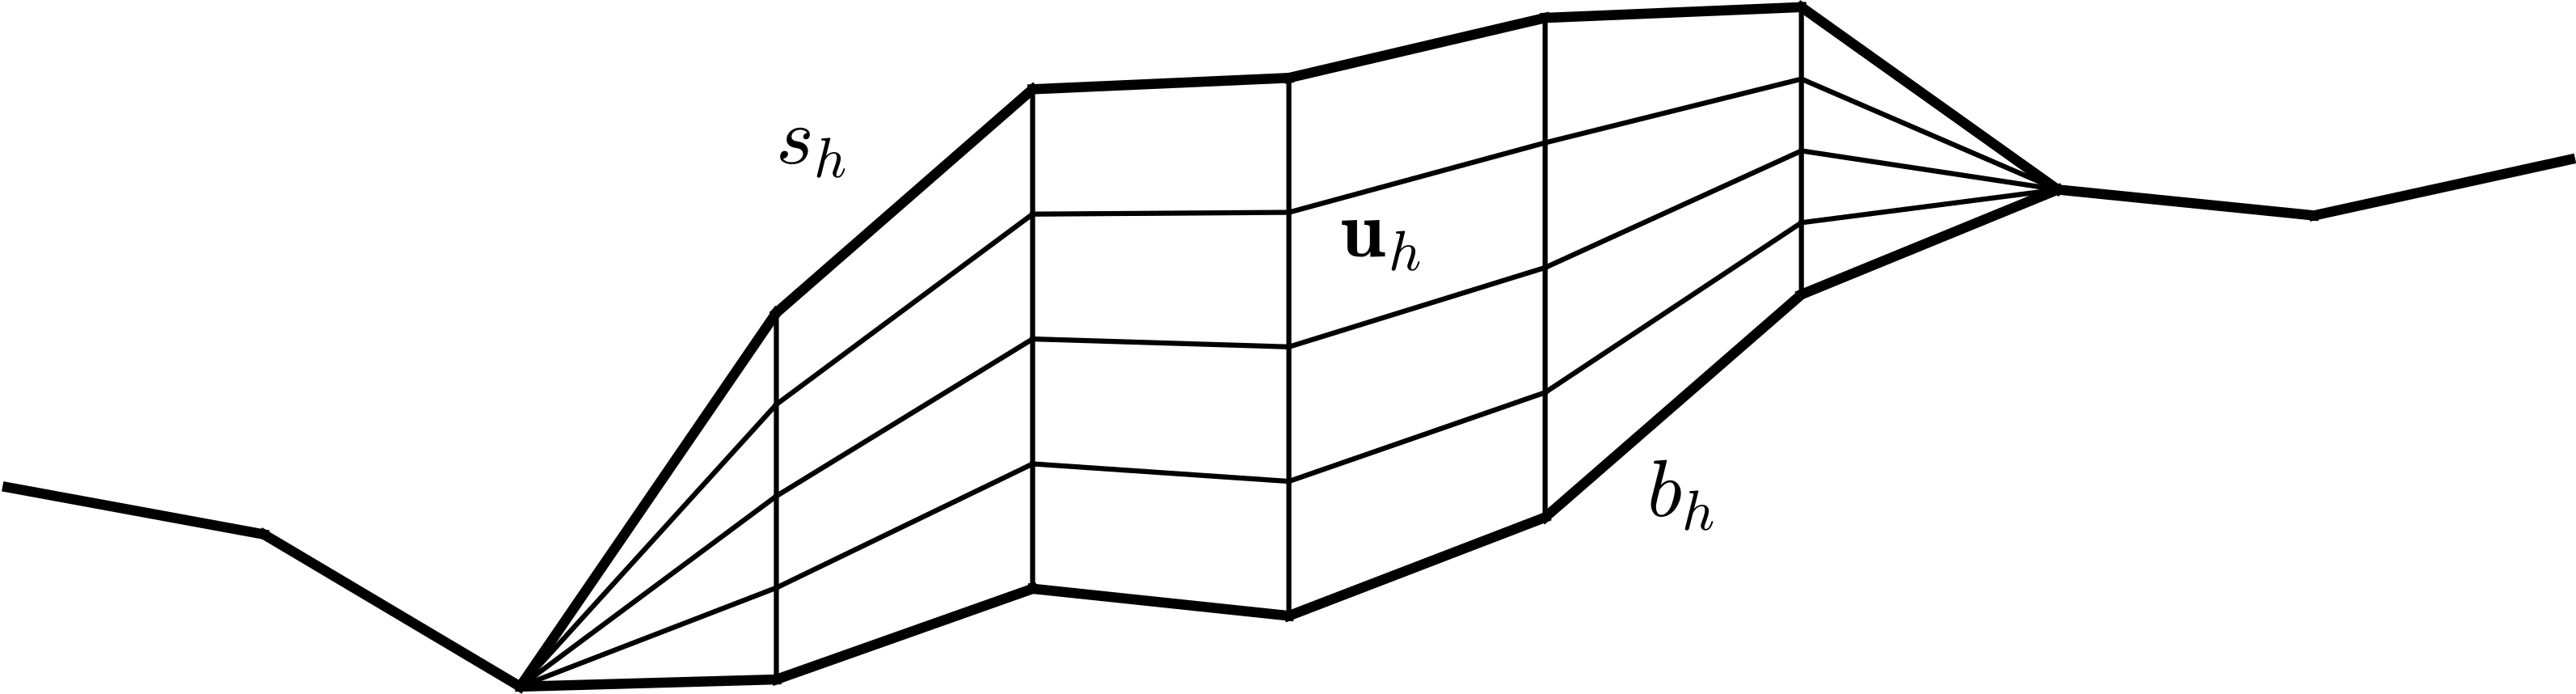
\includegraphics[width=0.7\textwidth]{genfigs/extruded.pdf}
\end{center}
\caption{Evaluating $F^h_{\Delta t}(s_h)$ in \eqref{eq:fe:be:Fdefine} requires numerically solving a Stokes problem for the velocity $\bu_h$, on a mesh between $b_h$ and $s_h$, and then evaluating its surface trace $\bu_h|_{s_h}$.}
\label{fig:fe:operatorvisualization}
\end{figure}

A key concern in applying abstract Theorem \ref{thm:abstractestimate}, or its Corollaries to the glacier problem is the choice of the numerical bed elevation $b_h \approx b$, which defines the constraint set $\cK_h$.  We will assume that $b$ is continuous on the closed domain $\bar\Omega$, i.e.~$b\in C(\bar\Omega) \cap \cX$.  In practice $b$ is provided via a high resolution map derived from ice-penetrating radar \cite{Morlighemetal2017}, and it may already be in a continuous FE space, but often it is on a finer mesh than $\cT_h$.  We assert that it is desirable to choose $b_h \in \cX_h$ to satisfy $b_h\ge b$ because the ``$\inf_{v\in\cK}$'' term in \eqref{eq:abstractestimate} disappears; see Corollary \ref{cor:abstractestimate:nohull}.  A monotone nodal operator \eqref{eq:monotoneop}, or similar, can be applied to achieve this, $b_h = R^\oplus b$.  As one would in a conforming FE method for a PDE problem \cite{Elmanetal2014}, we will assume $b_h=b$ along the fixed boundary $\partial\Omega$.  We also need to define an interpolation and truncation operation $\Pi_h : \cX \to \cK_h$ as follows.  For $r\in\cX$ this gives the unique FE function $\Pi_h(r) \in \cX_h$ so that
\begin{equation}
\Pi_h(r)(x_j) = \max \,\{b_h(x_j), r(x_j)\} \label{eq:definePi}
\end{equation}
for every interior node $x_j \in \cT_h$, with $\Pi_h(r)(x_j)=b(x_j)$ if $x_j\in\partial\Omega$.  Observe that definition \eqref{eq:definePi} only yields nodal admissibility.  The FE space must be such that this implies admissibility \emph{per se}, namely that $\Pi_h(r)(x) \ge b_h(x)$ for all $x \in \Omega$, so that $\Pi_h(r) \in \cK_h$.  This condition is satisfied by the continuous and piecewise-linear FE space $P_1$, but not, for example, by $P_2$ \cite{BuelerFarrell2024}, but compare the higher-order approach to FE solutions of VIs in \cite{KeithSurowiec2023}.

Collecting the above, from now on we make the following standard assumptions when solving VI problem \eqref{eq:be:vi} using numerical scheme \eqref{eq:fe:be:vi}.

\begin{stdass}
The following data are given:
\renewcommand{\labelenumi}{\arabic{enumi}.}
\begin{enumerate}
\item A bounded, convex polygon $\Omega\subset\RR^2$.
\item An exponent $\rr > 2$, with conjugate exponent $\rr' = \rr/(\rr-1)$. \label{item:rr}
\item A time-dependent SMB function $a\in C([0,T]; L^{\rr'}(\Omega))$.
\item A bed topography function $b \in C(\bar\Omega) \cap W^{1,\rr}(\Omega)$, with piecewise-linear boundary values $b|_{\partial\Omega}$.
\end{enumerate}
We make these definitions:
\begin{enumerate}
\setcounter{enumi}{4}
\item $\cX = W^{1,\rr}(\Omega)$, with the norm as defined in \eqref{eq:norm:Omega}.
\item $\cK = \{r\in\cX\,:\,r|_{\partial \Omega} = b|_{\partial \Omega} \text{ and } r \ge b\}$.
\end{enumerate}
The following are assumed to hold for the continuum problem:
\begin{enumerate}
\setcounter{enumi}{6}
\item Conjecture \ref{conj:a}. \label{item:conj:a}
\item Conjecture \ref{conj:b}. \label{item:conj:b}
\item Conjecture \ref{conj:c}, with exponent $\qq>1$ and coercivity constant $\alpha > 0$.\label{item:conj:c}
\end{enumerate}
We also assume and define for the FE method:
\begin{enumerate}
\setcounter{enumi}{9}
\item $\cT_h$ is a triangulation or quadrilateralization of $\bar\Omega$.
\item $\cX_h \subset \cX$ is a finite-dimensional and conforming FE space based on $\cT_h$.
\item $b_h\in\cX_h$ is given, with $b_h\ge b$ on $\bar\Omega$ and $b_h=b$ along $\partial \Omega$. \label{item:goodbh}
\item $\cK_h = \{r_h\in\cX_h\,:\,r_h|_{\partial \Omega} = b_h|_{\partial \Omega} \text{ and } r_h \ge b_h\}$. \label{item:defineKh}
\item The interpolation and truncation operator $\Pi_h:\cX \to \cK_h$ given by \eqref{eq:definePi}.  \label{item:Pi}
\end{enumerate}
\end{stdass}

\medskip
The conforming condition $\cK_h\subset \cK$ follows from assumptions \ref{item:goodbh} and \ref{item:defineKh}, with advantages to follow.  Note that defining $b_h=R^{\oplus} b$ implies assumption \ref{item:goodbh}, but we do not require this particular construction.  As seen in the proof of Theorem \ref{thm:regularizedwellposed}, assumptions \ref{item:conj:a} and \ref{item:conj:b} show that $F_{\Delta t}$ is $\qq$-coercive and Lipschitz on bounded subsets of $\cK$.  By case \emph{i)} of Corollary \ref{cor:abstractestimate:nohull} we have the following Lemma.

\begin{lemma} \label{lem:preglacierapp}  Make the Standard Assumptions.  Suppose that $s^{n-1}\in\cK$ and define $\ell^n \in \cX'$ by \eqref{eq:be:source}.  Let $s\in\cK$ be the unique surface elevation satisfying the implicit time-step VI problem \eqref{eq:be:vi}, from Theorem \ref{thm:regularizedwellposed}.  Assume that $s_h\in\cK_h$ solves problem \eqref{eq:fe:be:vi}.  Let $R_h=\max\{\|s\|_\cX,\|s_h\|_\cX\}$ and $\qq'=\qq/(\qq-1)$.  Then there is a constant $c_0>0$, depending on $R_h$ and $\Delta t$, but not otherwise on $s$ or $s_h$, so that
\begin{align}
\|s-s_h\|_\cX^\qq &\le \quad \frac{2}{\alpha \Delta t} \inf_{r_h\in\cK_h} \left(F_{\Delta t}(s)-\ell^n\right)[r_h-s] \label{eq:preglacierestimate} \\
   &\quad\, + \frac{2}{\alpha \Delta t} \left(F_{\Delta t}(s_h)-F^h_{\Delta t}(s_h)\right)[s_h] \notag \\
   &\quad\, + c_0 \inf_{r_h\in\cK_h} \|r_h - s\|_{\cX}^{\qq'}. \notag
\end{align}
\end{lemma}

Each term in bound \eqref{eq:preglacierestimate} turns out to have a clear meaning for glacier simulations, which we expose next.  Recall that $h$ denotes the maximum diameter of cells in $\cT_h$, $\Lambda(s_h)$ denotes the 3D domain defined by $s_h$ using \eqref{eq:icydomain}, $\cV=W_0^{1,\pp}(\Lambda(s_h); \RR^3)$ is the velocity space for the Stokes problem \eqref{eq:glenstokes:weak}, and $\tau_\pp(\Lambda(s_h))$ denotes the trace constant of domain $\Lambda(s_h)$ (Lemma \ref{lem:trace}).

\begin{theorem} \label{thm:glacierapp}  Make the same assumptions as in Lemma \ref{lem:preglacierapp}.  Define
\begin{equation}
\Omega_A(s) = \left\{x\in\Omega\,:\,s(x)=b(x)\right\},
\end{equation}
the active set for $s$, which is the ice-free region for the exact solution.  Then
\begin{align}
\phantom{dfkljsd} \|s_h-s\|_\cX^\qq &\le \quad \frac{2}{\alpha \Delta t} \int_{\Omega_A(s)} (b - \ell^n) (b_h - b) &&\text{\textnormal{[term 1]}} \label{eq:glacierestimate} \\
   &\quad\, + c(s_h) \big\|\bu_h - \bu\big\|_{\cV} &&\text{\textnormal{[term 2]}} \notag \\
   &\quad\, + c_0 \|\Pi_h(s) - s\|_\cX^{\qq'}, &&\text{\textnormal{[term 3]}} \notag
\end{align}
where $c_0>0$ is from Lemma \ref{lem:preglacierapp}.  The coefficient in term 2,
\begin{equation}
c(s_h) = \frac{C}{\alpha} \left(|\Omega| + [L]^{-\rr}\|s_h\|_{\cX}^\rr\right)^{1/(\pp'\rr)} \|s_h\|_{L^{\pp'\rr'}},
\end{equation}
depends nontrivially on $s_h$.
\end{theorem}

Before proving the Theorem we sketch the meaning of each term.  Further discussion happens after the proof.

\medskip
\begin{itemize}
\item[term 1:]  This term comes from FE approximation of the bed in the ice-free area $\Omega_A(s)$.  If the bed is exactly represented ($b_h=b$) then it is zero.  Note that $s_h \ge b_h \ge b = s$ in the ice-free area $\Omega_A(s)$, so the factor $b_h-b$ is the smaller than the difference $s_h - s$.  Because $b-\ell^n\ge 0$ (Section \ref{sec:model}), the integrand is nonnegative.

\item[term 2:]  This term quantifies how numerical velocity errors over the domain $\Lambda(s_h)$, from solving Stokes problem \eqref{eq:glenstokes:weak}, affect the numerical surface elevation error.

\item[term 3:]  An interpolation error term like this arises in the classical Cea's lemma argument for quasi-optimality of FE methods for PDEs \cite{Ciarlet2002}.  Here the interpolant of $s$ is interpolated \emph{and truncated} into $\cK_h$ using \eqref{eq:definePi}.
\end{itemize}

\begin{proof}  Because $s$ solves \eqref{eq:be:vi}, the residual $\Psi = F_{\Delta t}(s)-\ell^n \in \cX'$, while generally nonzero, is non-negative.  In fact, if $\phi\in C_c^\infty(\Omega)$ is nonnegative then $r=s+\phi \in \cK$ and $\Psi[r-s] = \Psi[\phi] \ge 0$.  Thus $\Psi\in\cX'$ is a non-negative distribution, and so it is represented by a positive Borel measure $\mu$ \cite[Theorem 6.22]{LiebLoss1997}, that is, $\Psi[\phi] = \int_\Omega \phi\,d\mu$.  However, by the proof of Theorem II.6.9 in \cite{KinderlehrerStampacchia1980} this measure is supported in $\Omega_A(s)$, and in fact it has density $b-\ell^n$ (Section \ref{sec:model}).

Now apply Lemma \ref{lem:preglacierapp}.  Note that $\bu|_{s}=\bzero$ and $s=b$ on $\Omega_A(s)$.  In the first term in \eqref{eq:preglacierestimate}, set $r_h = b_h \in \cK_h$ to give term 1:
\begin{equation}
\left(F_{\Delta t}(s)-\ell^n\right)[r_h-s] = \int_\Omega (b_h - s) \,d\mu = \int_{\Omega_A(s)} \left(b - \ell^n\right) (b_h - b).
\end{equation}
Consider the second term in \eqref{eq:preglacierestimate}.  Recall that $dS = |\bn_{s_h}|\,dx$ is the surface area element for the surface $\Gamma_{s_h} \subset \partial \Lambda(s_h)$.  After definitions \eqref{eq:be:Fdefine} and \eqref{eq:fe:be:Fdefine}, apply the triangle and H\"older inequalities:
\begin{align}
\left(F_{\Delta t}(s_h)-F^h_{\Delta t}(s_h)\right)&[s_h] = - \Delta t \int_\Omega \left(\bu|_{s_h} - \bu_h|_{s_h}\right)\cdot \bn_{s_h} s_h  \\
  &\le \Delta t \int_\Omega \Big|\bu|_{s_h} - \bu_h|_{s_h}\Big| |\bn_{s_h}|^{1/\pp} |\bn_{s_h}|^{1/\pp'} |s_h| \notag \\
  &\le \Delta t \left(\int_\Omega \Big|\bu|_{s_h} - \bu_h|_{s_h}\Big|^\pp |\bn_{s_h}|\right)^{1/\pp} \left(\int_\Omega |\bn_{s_h}| |s_h|^{\pp'}\right)^{1/\pp'} \notag \\
  &\le \Delta t \left(\int_{\Gamma_{s_h}} \big|\bu - \bu_h\big|^\pp dS\right)^{1/\pp} \left(\int_\Omega |\bn_{s_h}|^\rr\right)^{1/(\pp'\rr)} \|s_h\|_{L^{\pp'\rr'}} \notag
\end{align}
Now apply the trace inequality (Lemma \ref{lem:trace}) and use the facts that $\rr>2$ and $(1+\alpha)^{\rr/2} \le 2^{(\rr-2)/2} (1+\alpha^{\rr/2})$ if $\alpha\ge 0$:
\begin{align}
\left(F_{\Delta t}(s_h)-F^h_{\Delta t}(s_h)\right)[s_h] &\le \Delta t \left(\frac{\tau_\pp(\Lambda(s_h))}{[H]}\right)^{1/\pp} \|\bu - \bu_h\|_{\cV} \\
  &\qquad \cdot \left(2^{(\rr-2)/2} \int_\Omega 1 + |\grad s_h|^\rr\right)^{1/(\pp'\rr)} \|s_h\|_{L^{\pp'\rr'}}.  \notag
\end{align}
Recalling norm definition \eqref{eq:norm:Omega}, we have term 2.  Term 3 follows by substituting $r_h=\Pi_h(s)$ into the last term in \eqref{eq:preglacierestimate}.
\end{proof}

Regarding term 1, consider those portions of $\Omega_A(s)$ which are also ice-free according to the FE solution, namely points $x \in \Omega_A(s) \cap \Omega_A^h(s_h)$ where $\Omega_A^h(s_h) = \{x\in\Omega\,:\,s_h(x)=b_h(x)\}$.  In such areas generally $b_h > b$, for example because of the monotone restriction used for assumption \ref{item:goodbh}.  This implies that there is a positive ``fake ice thickness'' error for the FE solution, namely $s_h - b=b_h-b>0$.  However, the numerical model reports zero thickness ($s_h-b_h=0$).  In areas of strong ablation, and far from the nearest flowing glacier, one might simply declare that such ``fake ice'' does not represent an FE-generated error.  Then the magnitude of term 1 can be reduced accordingly, by excluding obviously ice-free areas from the integral.  However, generally $s$, and thus $\Omega_A(s)$, is unknown.  In fact, such exclusion is apparently not implementable near the unknown free boundary $\Omega \cap \partial \Omega_A(s)$.

Note that any time-stepping FE solution of a fluid-layer VI problem like \eqref{eq:be:vi} commits a mass conservation error near the (unknown) exact free boundary, even when there is no difference between the exact and FE obstacles.  The mass conservation barrier theory in \cite{Bueler2021conservation} addresses this concern, in terms of the fluid layer thickness, thus in a case where the obstacle is the zero function, which has an exact FE representation.  While the theory in \cite{Bueler2021conservation} applies here as well, term 1 in bound \eqref{eq:glacierestimate} is new relative to the mass-conservation errors identified in \cite{Bueler2021conservation}.

Regarding term 2, the Stokes velocity error norm $\|\bu_h - \bu\|_{\cV}$ in \eqref{eq:glacierestimate} describes the error in solving problem \eqref{eq:glenstokes:weak} on a particular 3D domain $\Lambda(s_h)$.  If one supposes (counter-factually) that $\Lambda(s_h)$ would not change under 2D mesh refinement of $\Omega$, then one may use reasonable assumptions and existing techniques to derive a convergence rate for this term.  The following sketch from \cite[Theorem 4.9]{JouvetRappaz2011} does this; see also the FE theory for linear Stokes in \cite{Elmanetal2014}:  One assumes solution regularity for the Stokes problem \eqref{eq:glenstokes:weak}, specifically that $\bu\in W^{2,\kappa}(\Lambda(s_h);\RR^3)$ and $p \in W^{1,\kappa'}(\Lambda(s_h))$ for some $\kappa \in [\pp,2]$.  The mixed FE method for \eqref{eq:glenstokes:weak} is assumed to satisfy Bramble-Hilbert interpolation bounds in $W^{1,\kappa}(\Lambda(s_h))$ and $L^{\kappa'}(\Lambda(s_h))$ for the discrete velocity and pressure spaces, respectively; see \cite[inequalities (4.26), (4.27)]{JouvetRappaz2011}.  Finally one assumes that the mixed FE method satisfies a discrete inf-sup condition \cite[equation (4.1)]{JouvetRappaz2011}.  One then concludes with a convergence rate, $\|\bu_h - \bu\|_{\cV} \le C h^{\kappa/2}$, for a constant $C>0$ which depends on the regularity norms of $\bu,p$, the discrete inf-sup constant, and the domain $\Lambda(s_h)$.

However, to apply such a technique to bounding term 2 of \eqref{eq:glacierestimate}, in the actual context of VI problem \eqref{eq:be:vi}, one would at least need to prove two new bounds.  First, one would need a bound showing the regularity of the solution $\bu,p$ of \eqref{eq:glenstokes:weak}, over the domain $\Lambda(s_h)$, when $s_h \in \cX_h \subset W^{1,\rr}(\Omega)$; this extends Conjecture \ref{conj:a}.  Second, seemingly much more difficult, one would need to bound how the constant in the convergence rate ``$C h^{\kappa/2}$'' (previous paragraph) depends on $\Lambda(s_h)$, that is, on $s_h$.

One might also try to bound term 3 in \eqref{eq:glacierestimate} via estimates for FE interpolation.  From \cite[Theorem 3.1.6]{Ciarlet2002}, for example, if $\mu \in [\rr,+\infty]$ then there is $C>0$, depending on $\Omega$ and the FE space $\cX_h$, such that for all $r \in W^{2,\mu}(\Omega)$, we have $\|\pi_h(r) - r\|_{\cX} \le C h \|r\|_{W^{2,\mu}}$.  Here $\pi_h$ is the ordinary interpolation into $\cX_h$, not including truncation into $\cK_h$ as in operation \eqref{eq:definePi}.  Now suppose we arrange that $\cK_h=\cK$, thus that $\Pi_h=\pi_h$, and suppose also that the exact solution $s\in\cK$ of VI problem \eqref{eq:be:vi} satisfies $s\in W^{2,\mu}(\Omega)$ for some $\mu \in [\rr,+\infty]$.  Then it follows that term 3 in \eqref{eq:glacierestimate} is $O(h)$ with a coefficient that depends on the $W^{2,\mu}$ norm of $s$.  The argument for \cite[Theorem 4.3]{JouvetBueler2012} makes a comparably-strong regularity assumption for a power of the thickness function in an SIA problem.

However, the sketch in the previous paragraph is largely a fantasy.  The hypothesis that $s\in W^{2,\mu}(\Omega)$ is too strong even if the data $a,b$ entering into VI problem \eqref{eq:be:vi} are arbitrarily smooth.  While it is true that in classical obstacle problems the solution is generically tangential along the free boundary, which permits such regularity \cite[Chapter IV]{KinderlehrerStampacchia1980}, here a glacier's surface gradient need not approach the bed gradient at points along the ice margin.  Thus, while $s \in \cX = W^{1,\rr}(\Omega)$ is credible, $s\in W^{2,\mu}(\Omega)$ is probably not.  This sketch suggests that direct use of standard FE interpolation theory to prove convergence via a result like Theorem \ref{thm:glacierapp} would seem to be difficult.


\section{Discussion and conclusion} \label{sec:conclusion}

We know of no existing literature of Stokes-based glacier geometry evolution which is mathematical in a comparable sense to this paper.  Specifically, a coupled weak form for the glacier evolution problem with Stokes dynamics, which is the only conceivable basis for rigorously addressing that problem, seems not to have appeared in the literature.  Nor has a Sobolev space for the surface elevation functions, in such a theory, been proposed.  However, numerical solvers for this, until now largely unstated, continuum problem are in wide-spread use for glacier modeling.

FIXME no results known to the author prove such well-posedness, \emph{nor for any glacier geometry evolution problem based on Stokes dynamics}

The major result of this paper is Theorem \ref{thm:glacierapp}, which bounds the numerical surface elevation error, in a single backward Euler time step, when a glacier is modeled using non-shallow Stokes dynamics.  The bound, inequality \eqref{eq:glacierestimate}, only estimates the FE error made in solving VI problem \eqref{eq:be:vi}.  The first two terms in the bound can be reduced by improved bed elevation interpolation, and by solving the Stokes problem more accurately, respectively.  All terms in the bound are reduced by increased mesh resolution over the fixed domain $\Omega\subset \RR^2$.  However, the surface elevation solution to \eqref{eq:be:vi} must be expected to have low regularity, especially across the ice margin (free boundary).  Near-margin mesh refinement may be the only technique which reduces the interpolation/truncation error in the surface elevation, namely term 3 in \eqref{eq:glacierestimate}.

The results here leave us far from an FE convergence proof for the main time-evolution problem of glaciology, which is the problem stated in the Introduction.  This problem couples NCP \eqref{eq:ncp} to the Stokes problem \eqref{eq:glen}--\eqref{eq:stokes}.  It seems to be a parabolic VI \cite{Glowinski1984}, on which analysis may be more difficult than for the (roughly-speaking) elliptic single-step VI problem \eqref{eq:be:vi}.  Converting Theorem \ref{thm:glacierapp} to a convergence proof for the time-dependent theory would require significant extensions.

We do not possess a proof of the well-posedness of the continuous-space, implicit-step problem \eqref{eq:be:vi} itself.  While part of the current paper is devoted to conjecturing such well-posedness (Sections \ref{sec:model}--\ref{sec:conjectural}), the abstract FE bound in Theorem \ref{thm:abstractestimate} applied to problem \eqref{eq:be:vi} is the main result, that is, Theorem \ref{thm:glacierapp}.  The abstract bound applies because of Theorem \ref{thm:regularizedwellposed}, a consequence of Conjectures \ref{conj:a}, \ref{conj:b}, and \ref{conj:c}.  The heart of the matter is coercivity of the surface motion, namely Conjecture \ref{conj:c}, but a strategy for proving this is not clear to this author.  Our results here at least clarify which properties of the surface motion, as part of a free-boundary problem for the surface kinematical equation, need to hold so that mathematically sensible time steps can be taken in a non-shallow glacier model.


%\clearpage\newpage
\bibliographystyle{siamplain}
\bibliography{estimate}

\appendix
\section{Proof of Lemma \ref{lem:stokesapriori}} \label{app:provestokesapriori}

The proof of Lemma \ref{lem:stokesapriori} is hinted in \cite{JouvetRappaz2011}, and is standard.  It requires Poincar\'e's inequality, below as \eqref{eq:poincare}, which is (7.44) in \cite{GilbargTrudinger2001}, and Korn's inequality \eqref{eq:korns}, which can by proven by setting $F(x)$ to the identity in Corollary 4.1 of \cite{Pompe2003}.

\begin{lemma} \label{lem:poincarekorns}
Under the assumptions of Theorem \ref{thm:stokeswellposed}, there exist dimensionless constants $C$, depending on the geometry of $\Lambda$, so that for all $\bv \in \cV$,
\begin{equation}
\int_\Lambda |\bv|^\pp \le C [H]^\pp \int_\Lambda |\grad\bv|^\pp, \label{eq:poincare}
\end{equation}
thus $\|\bv\|_{\cV}^\pp \le (C + 1) [H]^\pp \int_\Lambda |\grad\bv|^\pp$, and
\begin{equation}
\int_\Lambda |\grad\bv|^\pp \le C \int_\Lambda |D\bv|^\pp. \label{eq:korns}
\end{equation}
\end{lemma}

\begin{proof}[Proof of Lemma \ref{lem:stokesapriori}]
From \eqref{eq:glenstokes:weak} and $\bu \in\Vdiv$ it follows that
\begin{equation}
0= F_\Lambda(\bu,p)[\bu,p] = \int_\Lambda 2 \nu(D\bu) D\bu : D\bu - \rhoi \bg \cdot \bu.  \label{eq:stokes:substituteu}
\end{equation}
Apply \eqref{eq:korns}, the facts that $\pp>0$ and $(\pp-2)/2 \le 0$, and equation \eqref{eq:glen}:
\begin{align}
\int_\Lambda |\grad\bu|^\pp &\le C \int_\Lambda |D\bu|^\pp \le C \int_\Lambda \left(|D\bu|^2 + \eps\right)^{(\pp-2)/2} \left(D\bu:D\bu + \eps\right) \label{eq:stokes:startapriori} \\
	&= C \left[\eps^{\pp/2} |\Lambda| + (2 \nu_\pp)^{-1} \int_\Lambda 2\nu(D\bu) D\bu:D\bu\right]. \notag
\end{align}
By equation \eqref{eq:stokes:substituteu}, Cauchy-Schwarz, and H\"older's inequality we thus have
\begin{align}
\int_\Lambda |\grad\bu|^\pp &\le C \left[\eps^{\pp/2} |\Lambda| + (2 \nu_\pp)^{-1} \int_\Lambda \rhoi \bg \cdot \bu\right] \label{eq:stokes:workapriori} \\
	&\le C \left[\eps^{\pp/2} |\Lambda| + (2 \nu_\pp)^{-1} \rhoi |\bg| |\Lambda|^{1/\pp'} \|\bu\|_\cV\right]. \notag
\end{align}
From \eqref{eq:poincare},
\begin{equation}
\|\bu\|_{\cV}^\pp \le C [H]^\pp \left[\eps^{\pp/2} |\Lambda| + (2 \nu_\pp)^{-1} \rhoi |\bg| |\Lambda|^{1/\pp'} \|\bu\|_\cV\right].
\end{equation}
Now let $z=\|\bu\|_\cV$.  We have proved that $z^\pp \le c_0 + c_1 z$ for $\pp>1$ and constants $c_i>0$.  Furthermore $g(y) = y^\pp - c_1 y - c_0$ is smooth with $g(0)=-c_0<0$, and $g(y) \to +\infty$ as $y \to +\infty$ since $\pp>1$.  Thus there exists a right-most root $\tilde y>0$ with $\tilde y = f(\pp,c_0,c_1)$.  Since $g(z)\le 0$ we have $z \le \tilde y$.  This proves \eqref{eq:stokesapriori} with $C=\tilde y$.
\end{proof}


\section{The surface motion map is not coercive} \label{app:noncoercive}

It is reasonable to suppose that glacier flow models have the property that, for smooth bedrock elevations, there is no flow whenever an admissible surface elevation $s\in \cX=W^{1,r}(\Omega)$ is flat (horizontal) on the ice.  In terms of the inactive set $\Omega_I=\{x\in\Omega\,:\,s(x)>b(x)\}$ (Section \ref{sec:model}) and the 3D icy domain $\Lambda(s)$ (equation \eqref{eq:icydomain}) defined earlier, this property is that if $\grad s=0$ a.e.~in $\Omega_I$ then $\bu=\bzero$ on $\Lambda(s)$.  By well-posedness Theorem \ref{thm:stokeswellposed} this property holds for the (non-sliding) Stokes model considered in the paper.  However, it also holds for a Stokes model with any physically-reasonable sliding law, and for any shallow ice approximation model \cite{JouvetBueler2012}.

Using this property, for bedrock elevations $b$ which have strict local minima then we can construct distinct surface elevations $s_1,s_2\in \cX$, $\|s_1-s_2\|_{\cX}>0$, each with zero surface motion: $\bu|_{s_i}=\bzero$ and $\Phi(s_i)=0$.  (See \eqref{eq:defineus} and \eqref{eq:definePhi}.)  The construction (Figure \ref{fig:noncoercive}) is simply to fill the local minima with flat ice for surface $s_1$, and leave the other as bare ground $s_2=b$.  Note that $s_1$ can be constructed with any (positive) number of local minima filled-in, or with minima only partially filled, but again one has $s_1 \in \cX$, satisfying $\bu|_{s_1}=\bzero$, $\Phi(s_1)=0$, and $\|s_1-s_2\|_{\cX}>0$.

\begin{figure}[ht]
\begin{center}
\mbox{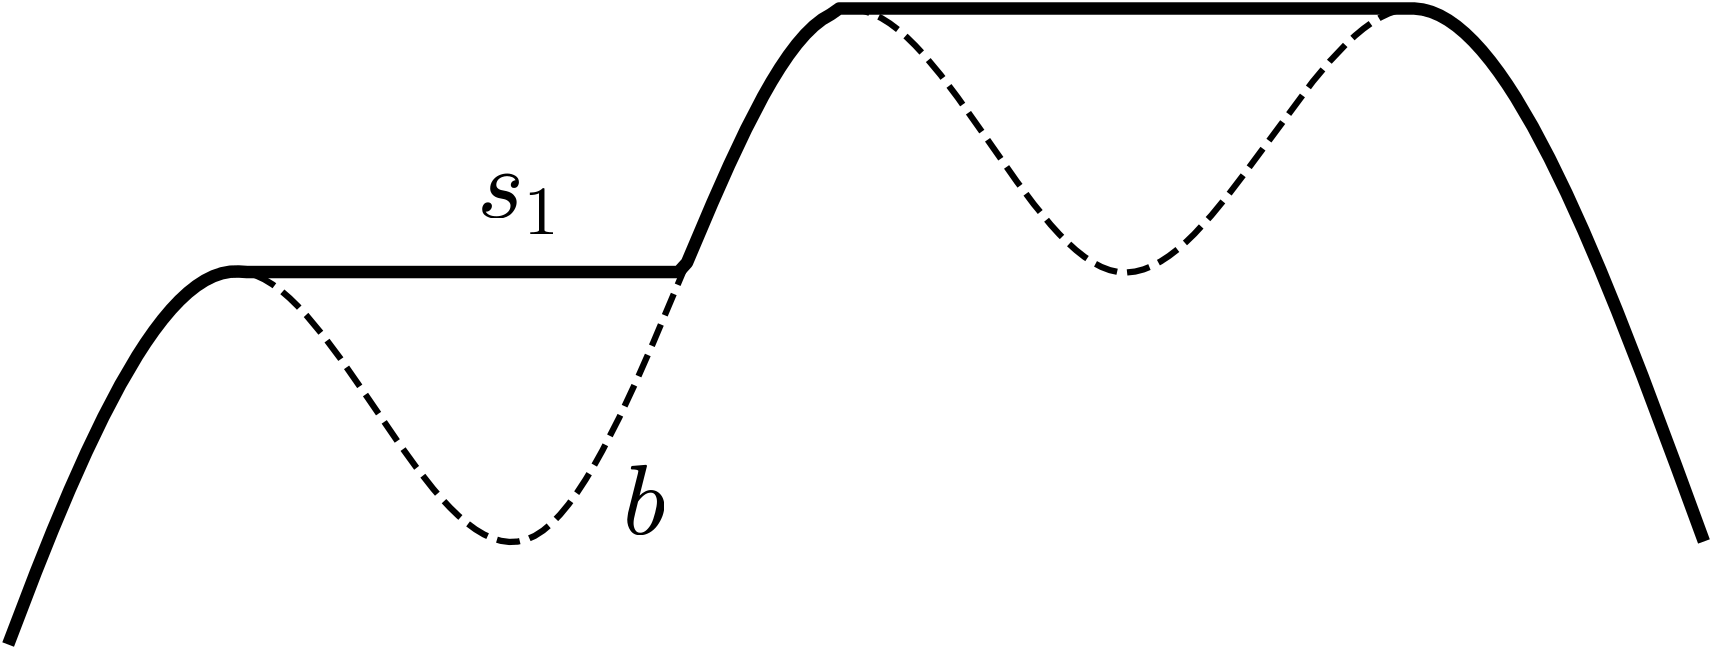
\includegraphics[width=0.4\textwidth]{genfigs/filled.pdf} \qquad 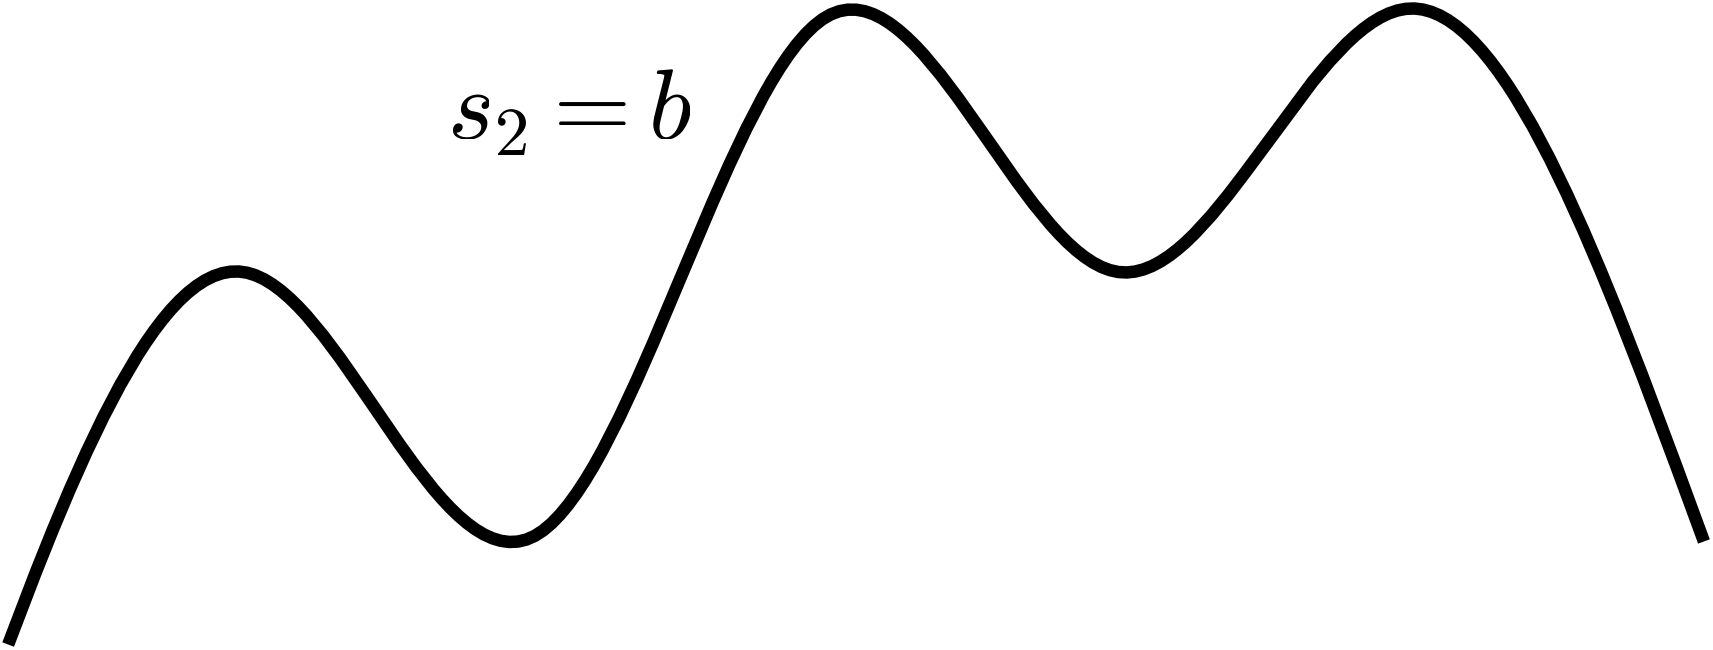
\includegraphics[width=0.4\textwidth]{genfigs/icefree.pdf}}
\end{center}
\caption{For a smooth bedrock elevation $b$ with local minima, a surface elevation state $s_1$ that fills-in the minima with flat ice (left) gives zero surface velocity in a Stokes model: $\bu|_{s_1}=\bzero$.   The ice-free state $s_2=b$ (right) likewise has $\bu|_{s_2}=\bzero$.  This shows that the surface motion map $\Phi$ defined in \eqref{eq:definePhi} is not coercive.}
\label{fig:noncoercive}
\end{figure}

Two consequences of this construction are now stated as propositions.

\begin{proposition} \label{prop:noncoercive}
The surface motion map $\Phi$ defined in \eqref{eq:definePhi} is not $q$-coercive (Definition \ref{def:monotonecoercive}), for any $q$, nor is it strictly-monotone.
\end{proposition}

\begin{proof}
Note $(\Phi(s_1) - \Phi(s_2))[s_1-s_2]=0$ while $\alpha \|s_1-s_2\|_\cX > 0$.
\end{proof}

\begin{proposition} \label{prop:notunique}
When the SMB is identically zero, $a=0$, there are smooth bedrock elevations for which the steady-state version of a glacier geometry model will have more than one solution.
\end{proposition}

\begin{proof}
The NCP form of the steady-state and $a=0$ model in question is
	$$s - b \ge 0, \quad - \bu|_s \cdot \bn_s \ge 0, \quad (s - b) \left(- \bu|_s \cdot \bn_s\right) = 0,$$
with corresponding weak form over $s\in\cK\subset\cX$.  If $b$ is a smooth function with local minima then the above construction of $s_1$ and $s_2$ gives distinct solutions.
\end{proof}
Proposition \ref{prop:notunique} answers negatively the uniqueness question which has been open since the existence theorem for the general-bed, steady shallow ice approximation \cite{JouvetBueler2012}.  It uses a surprisingly-simple construction, but one which seems not to appear in the literature.  Non-uniqueness here happens for a SMB function which is elevation \emph{in}dependent, namely $a=0$.  This result is different from the better-known non-uniqueness \cite{Bodvardsson1955} and non-existence \cite{Jouvetetal2011} results for certain elevation-dependent SMB models.


\section{Numerical experiments on the surface motion map} \label{app:numerical}

FIXME make shorter; histograms without and then with $p$-Laplacian regularization

We may explore the validity of Conjecture \ref{conj:b} by sampling from numerical simulations.  The experiments here,\footnote{Source code is at the public repository \href{https://github.com/bueler/glacier-fe-estimate}{\texttt{github.com/bueler/glacier-fe-estimate}}, in the \texttt{py/} directory.  The codes call the library at \href{https://github.com/bueler/stokes-extrude}{\texttt{github.com/bueler/stokes-extrude}}.} performed using Python and the Firedrake FE library \cite{Hametal2023}, are not intended to demonstrate implicit time-stepping, but only to generate admissible surface elevation pairs $r,s\in\cK$ to use as samples.  For a given sample pair we evaluate the $2$-coercivity ratio
\begin{equation}
\rho(r,s) = \frac{\left(\Phi(r) - \Phi(s)\right)[r-s]}{\|r-s\|_{\cX}^2}. \label{eq:Phiratio}
\end{equation}
If, for all pairs in some $\cK$, the set of ratios $\{\rho(r,s)\}$ were bounded below by a positive constant $\alpha>0$, then this would confirm the $\qq=2$ coercivity inequality \eqref{eq:conj:c} for that $\cK$.  Of course, a numerical experiment allows only finite sampling, and furthermore a finite spatial discretization must be used.

The domain for our experiments is the 1D interval $\Omega=(-L,L)$, $L=100$ km, with $\cX = W_b^{1,2}(\Omega)$.  The interval $\Omega$ was uniformly-meshed into equal intervals.  The $P_1$ piecewise-linear FE space $\cX_h\subset \cX$ was used for the bed $b$ and the surface $s$, giving polygonal domains $\Lambda$ defined by $b,s$; see equation \eqref{eq:icydomain}.  Three bed profiles  (Figure \ref{fig:cases}) were considered, \emph{flat} with $b=0$, \emph{smooth} with a superposition of several wavelengths down to 10 km, and \emph{rough} with an additional 4 km wavelength mode.  These beds generate corresponding constraint sets $\cK_i \subset \cX$, $i=1,2,3$.  For each constraint set $\cK_i$, three constant SMB values were considered (units $\text{m}\,\text{s}^{-1}$): $a\in\{-2.5,0.0,1.0\}\times 10^{-7}$.  For each SMB value a time-dependent run of duration $T=200$ years started from the same initial surface elevation profile.\footnote{A Halfar profile \cite{Halfar1981} with characteristic time $t_0=29$ years was used as the initial state.  In the case of a flat bed and $a=0$ the exact time-dependent solution under SIA dynamics is known by Halfar's result \cite{Halfar1981}, so the final surface elevation, from using Stokes dynamics in the numerical experiment, agrees closely with the SIA exact solution; compare comments in \cite{LofgrenAhlkronaHelanow2022}.}  The positive SMB value was sufficient to advance the ice margins nearly to the domain boundary at $|x|=L$ by the final time $T$, while the negative SMB value caused the glacier to disappear entirely by that time.

\begin{figure}[ht]
\mbox{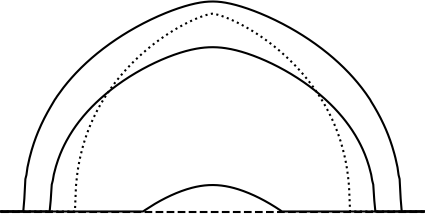
\includegraphics[width=0.30\textwidth]{figs/snapsflat.png} \, 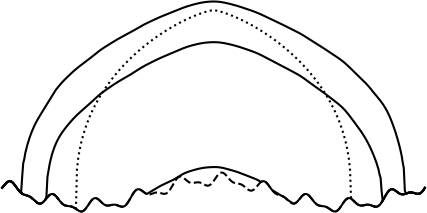
\includegraphics[width=0.32\textwidth]{figs/snapssmooth.png} \, 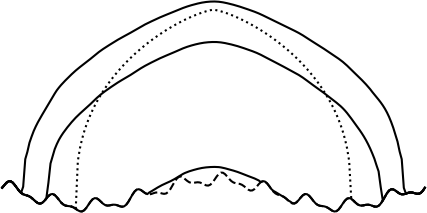
\includegraphics[width=0.32\textwidth]{figs/snapsrough.png}}

\caption{Three bed cases (flat, smooth, rough) define constraint sets $\cK_i\subset\cX$ in the numerical experiment.  For each $\cK_i$, three time-dependent runs of $T=200$ years, starting from the same initial state (dotted), but using different constant values of the SMB (see text), generated a large number of admissible states.  Example states at $t=170$ years are shown (solid).  Ratios \eqref{eq:Phiratio} were computed for 1000 sample pairs $r,s$ from each set $\cK_i$.}
\label{fig:cases}
\end{figure}

In these simulations each time-step VI \eqref{eq:be:vi} was done semi-implicitly.  That is, definition \eqref{eq:be:Fdefine} was modified to use the prior surface velocity $\bu|_{s^{n-1}}$.  The numerical VI solution was by a reduced-space Newton method with line search \cite{BensonMunson2006}.  The ``FSSA'' stabilization technique from \cite{LofgrenAhlkronaHelanow2022} was applied, which generates a modified Stokes weak form compared to \eqref{eq:glenstokes:weak}; see equation (23) in \cite{LofgrenAhlkronaHelanow2022}.  The Stokes problem \eqref{eq:glenstokes:weak}, with viscosity regularization $\eps=10^{-19}\, \text{s}^{-2}$ in \eqref{eq:glen}, was solved on each domain $\Lambda$ using a vertically-extruded mesh of quadrilaterals (Figure \ref{fig:fe:operatorvisualization}), mixed FE method for the $Q_2\times Q_1$ (Taylor-Hood) stable pair \cite{Elmanetal2014}, and a Newton solver, with direct solution of the linear step equations.  The resulting time-dependent numerical method is only conditionally stable, but adequate for our purpose of generating sample surfaces.

The basic result of these experiments is shown in Figure \ref{fig:ratios}.  These are sample ratio $\rho(r,s)$ histograms from the highest spatial resolution, namely $\Delta x=500$ m and 40 elements in each extruded column.  More than $87\%$ of all the ratios were positive, and of these the medians for the three $\cK_i$ were in the range $[4.5,5.2] \times 10^{-13}$.  For the remaining negative ratios, the medians were in the range $[-4.1,-2.8]\times 10^{-14}$, much smaller in magnitude.

\begin{figure}[ht]
\mbox{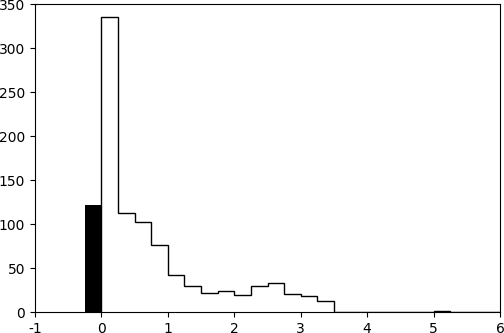
\includegraphics[width=0.32\textwidth]{figs/flatratios.png} \, 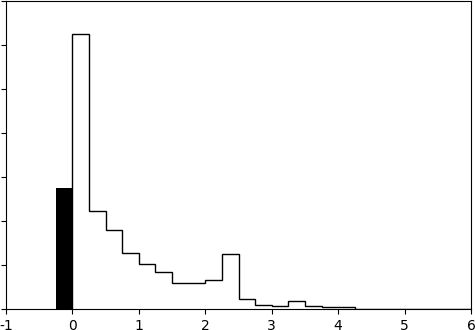
\includegraphics[width=0.30\textwidth]{figs/smoothratios.png} \, 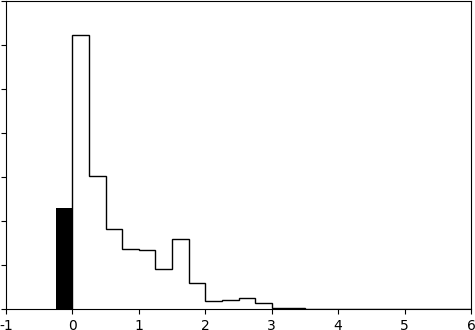
\includegraphics[width=0.30\textwidth]{figs/roughratios.png}}

\caption{Histograms of ratios $\rho(r,s)$ for 1000 sample pairs from each of the three sets $\cK_i$ (Figure \ref{fig:cases}).  The horizontal axis has  $\rho(r,s) \in [-1,6]\times 10^{-12}$, and the common vertical axis is for counts between 0 and 350.  About $10\%$ of these ratios are negative (solid).}
\label{fig:ratios}
\end{figure}

Figure \ref{fig:ratios} does \emph{not} represent compelling evidence of $2$-coercivity by definition \eqref{eq:qcoercive}, but it does not exclude it.  In fact, the details of the discretization of the ice margin strongly influence the negative ratios.  Noting that ratio evaluation uses integral \eqref{eq:definePhi}, if that integrand is reset to zero where the ice is thinner than 100 m then the negative values disappear (not shown).  Even without such thresholding, at lower horizontal resolution ($\Delta x=2000$ m) the median magnitude of negative ratios was roughly twice as large (not shown).  The disappearance of negative ratios under grid refinement therefore should not be excluded.  Margin approximation improvements, such as adaptive/local mesh refinement, will probably improve the numerical evidence for $2$-coercivity.

It is theoretically possible that the operator $\Phi$ is monotone---see inequality \eqref{eq:monotone}---but not $\qq$-coercive for any $\qq$.  In that case a revised well-posedness argument can be attempted, for example by adding a small coercive form as in section III.2 of \cite{KinderlehrerStampacchia1980}.  However, if a continuum pair $r,s$ with a negative ratio were actually to be found in some $\cK$, i.e.~with an exact continuum ratio $\rho(r,s)<0$ from \eqref{eq:Phiratio}, then the coercivity-based well-posedness framework of this paper would fail unless VI problem \eqref{eq:be:vi} is permanently regularized.

Regarding Conjecture \ref{conj:a}, i.e.~Lipschitz continuity for the surface velocity trace, the ratio $\big\|\bu|_r - \bu|_s\big\|_{L^2}/\|r-s\|_{W^{1,2}}$ for the same sample pairs was also evaluated.  Over all three sets $\cK_i$, at the highest resolution, the maximum ratio was $3.5\times 10^{-9}$, providing a lower bound for $C_A$.  Again, numerical experiments obviously cannot prove Conjecture \ref{conj:a}.


\end{document}
